\documentclass[11pt]{article}
\usepackage[utf8]{inputenc}
\usepackage[pdftex]{graphicx}
\usepackage{pdfpages}
\usepackage{makeidx}
\usepackage[english]{babel}
\usepackage [autostyle, english = american]{csquotes}
\usepackage{mathtools}
\usepackage{xcolor}
\usepackage{listings}
\usepackage{caption,subcaption}
%\usepackage{subfigure}
\usepackage{geometry}
\usepackage{adjustbox}
\usepackage{calc}
\usepackage{ifthen}
\usepackage{listings}
\usepackage{hyperref}
\usepackage{cleveref}
\usepackage[section,cachedir=build,newfloat]{minted}
\usepackage{chngcntr}
\usepackage[cm]{fullpage}

\definecolor{mintedbackground}{rgb}{0,0,0}


\usemintedstyle{tango}
\newenvironment{code}{\captionsetup{type=listing}}{}
\SetupFloatingEnvironment{listing}{name=Source Code}
\captionsetup[subfigure]{subrefformat=simple,labelformat=simple}

\renewcommand{\thelisting}{\arabic{listing}}
\renewcommand\thesubfigure{(\alph{subfigure})}

\bibliographystyle{abbrvnat}

\geometry{
 a4paper,
 total={170mm,257mm},
 left=10mm,
 right=10mm,
 top=10mm,
}

\graphicspath{ {code/} }

\definecolor{lightgray}{rgb}{.7,.7,.7}
\definecolor{gray}{rgb}{.4,.4,.4}
\definecolor{darkblue}{rgb}{0,0,.3}
\definecolor{gray}{rgb}{0.4,0.4,0.4}
\definecolor{darkblue}{rgb}{0.0,0.0,0.6}
\definecolor{cyan}{rgb}{0.0,0.6,0.6}

\lstset{
  basicstyle=\ttfamily,
  columns=fullflexible,
  showstringspaces=false,
  commentstyle=\color{gray}\upshape
}

\hypersetup{
    colorlinks,
    citecolor=black,
    filecolor=black,
    linkcolor=black,
    urlcolor=blue
}
 


\newmintedfile[pycode]{python3}{
frame=lines,
framesep=2mm,
fontsize=\footnotesize,
showtabs =false,
autogobble=true,
breaklines=true,
mathescape=true
}

\newmintedfile[rcode]{S}{
frame=lines,
framesep=2mm,
fontsize=\footnotesize,
showtabs =false,
autogobble=true,
breaklines=true,
mathescape=true
}

\title{Assignment 2 \\ Introduction to Information Retrieval \\ CS734/834}
\author{John Berlin}
\date{\today}
\renewcommand\thesection{Q.\arabic{section}}
\renewcommand\thesubsection{\thesection}
\begin{document}
\maketitle
\newpage
\section*{Note}
In order to make processing of the Wiki dataset timely and repeatable the util python file \autoref{code:util}, was utilized to serialize the files full paths to disk in \href{https://docs.python.org/3/library/pickle.html}{pickle} format. Also included in this serialization was a python set of Wiki articles for both small and large datasets. This is to ensure that self links were not included when doing the calculations for \autoref{q:pr}; also each question involving the Wiki dataset uses these file paths to read the html files for a given article. \newline \newline The pickle formated produced when answering the questions about the Wiki dataset are included with this report in tar.gz format if it did not exceed the file size restrictions enforced by Github. For more information concerning this please read this \href{https://help.github.com/articles/what-is-my-disk-quota/}{post} from Github. Graphv3 generated by \autoref{q:pr} is not included with this report as its size is 436mb compressed likewise the inverted index for wiki-large is not included as its size if 1.6gb uncompressed in pickle format. 

\section{Question 4.2}
\begin{verbatim}
Plot vocabulary growth for the Wikipedia collection and estimate the parameters 
for Heaps’ law. Should the order in which the documents are processed
make any difference?
\end{verbatim}
\subsection{Answer}
Processing of both the small and large Wiki articles was straight forward. 
Beautiful soup was used to extract the text from the articles as it removes the markup for you automatically. Each articles text was cleaned by replacing characters matched a regular expression looking for consecutive whitespace characters and punctuation (excluding punctuation that is included in valid words i.e \textit{John's})  with a single space character. Tokenization of an articles text was done using the WordPunctTokenizer provided by the nltk library. This tokenizer preserves the punctuation of the text hence the need for removing prior to tokenization. Tokens produced in tokenization that had a length of one were excluded in the vocabulary calculations. Each token that had length greater than one was counted towards the word count and if the token was not in the vocabulary set it was added increasing the vocabulary count by one. The code for this is seen in \autoref{code:vcp}. \newline

\noindent It must be noted that the counts used in the plots are when a new vocabulary item is found. This is due to the size of the files when counting every word. The  large data set produced a file of 1.4gb and the small produced a file sizes of 59mb.  \autoref{tb:vcd} shows the minute differences in the actual counts and that the size of the files is due to the repeated entries in them.
\begin{table}[h]
\centering
\caption{Vocab Count Differences}
\label{tb:vcd}
\begin{minipage}{.5\linewidth}
\begin{tabular}{lll}
Word Count & Vocab Count & File \\
4,090,585 & 232,028 & Small Vocab \\
4,090,629 & 232,028 & Small Vocab Full
\end{tabular}
\end{minipage}%
\begin{minipage}{.5\linewidth}
\begin{tabular}{lll}
Word Count & Vocab Count & File \\
82,961,568 & 1,526,042 & Large Vocab \\
82,961,616 & 1,526,042 & Large Vocab Full
\end{tabular}
\end{minipage}
\end{table}
\newline \newline Estimation of the parameters for heaps law and plotting was done in R and can be seen in \autoref{code:vcr}.  The parameters \textit{K} and \textit{B} were estimated using non-linear least squares (nls) method and both variables initially had values of one at the beginning of the calculation. Values produced by nls were plotted along side the values from the Wiki dataset on the y-axis as vocab count after using the predict method which is the goal of this question. I augmented the second part of this question by adding random order processing when building the vocabulary. This was to answer my own question about the order after plotting the in-order and reverse order plots. \newline \newline 
Heaps approximation was close for both the small and large \autoref{fig:wvg}. The real values followed the predicted for the first half then fluctuate for the remaining two quarters of the data set. The first fluctuation shows the point where the vocabulary grows slowly in comparison to the estimate. This plateau is due to the probability of actually seeing new words this far into data set. The second fluctuation can is an increase above the estimation and can be attributed to the data set having more non-English text as Japanese articles about Hyundai are included at the end.
\begin{figure}[h]
\centering
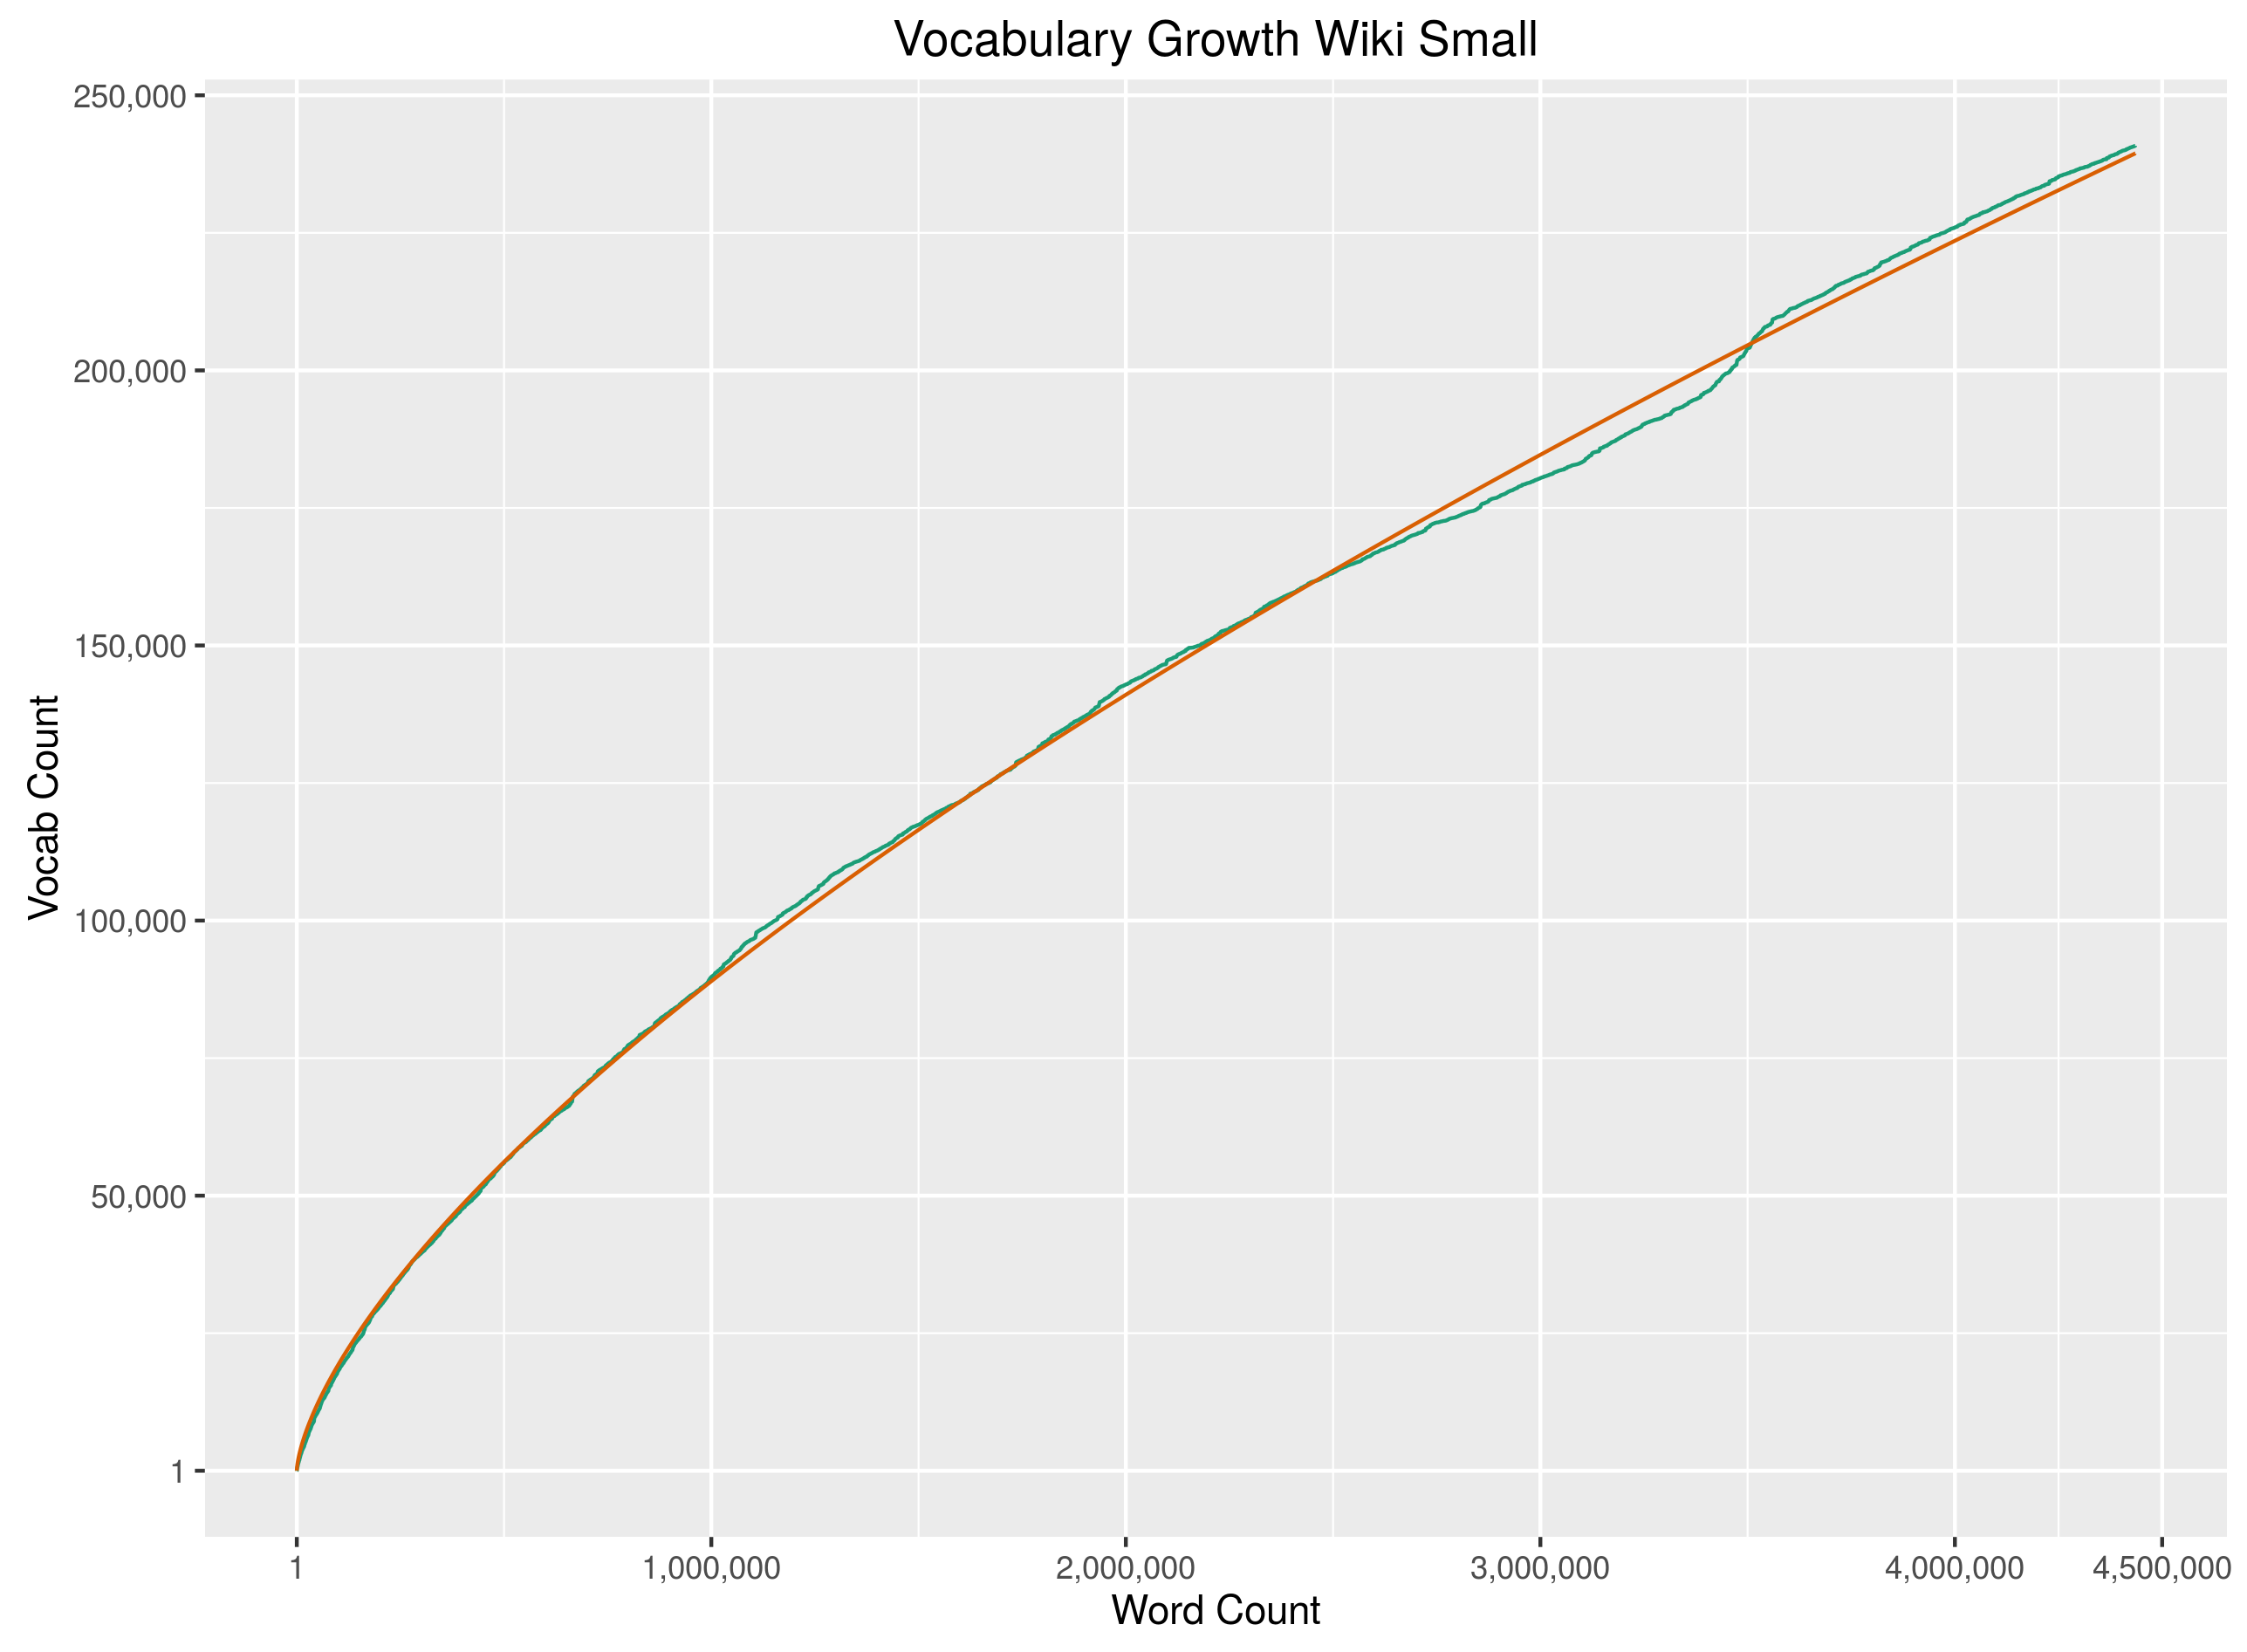
\includegraphics[scale=0.6]{wikiSmallVG.png}
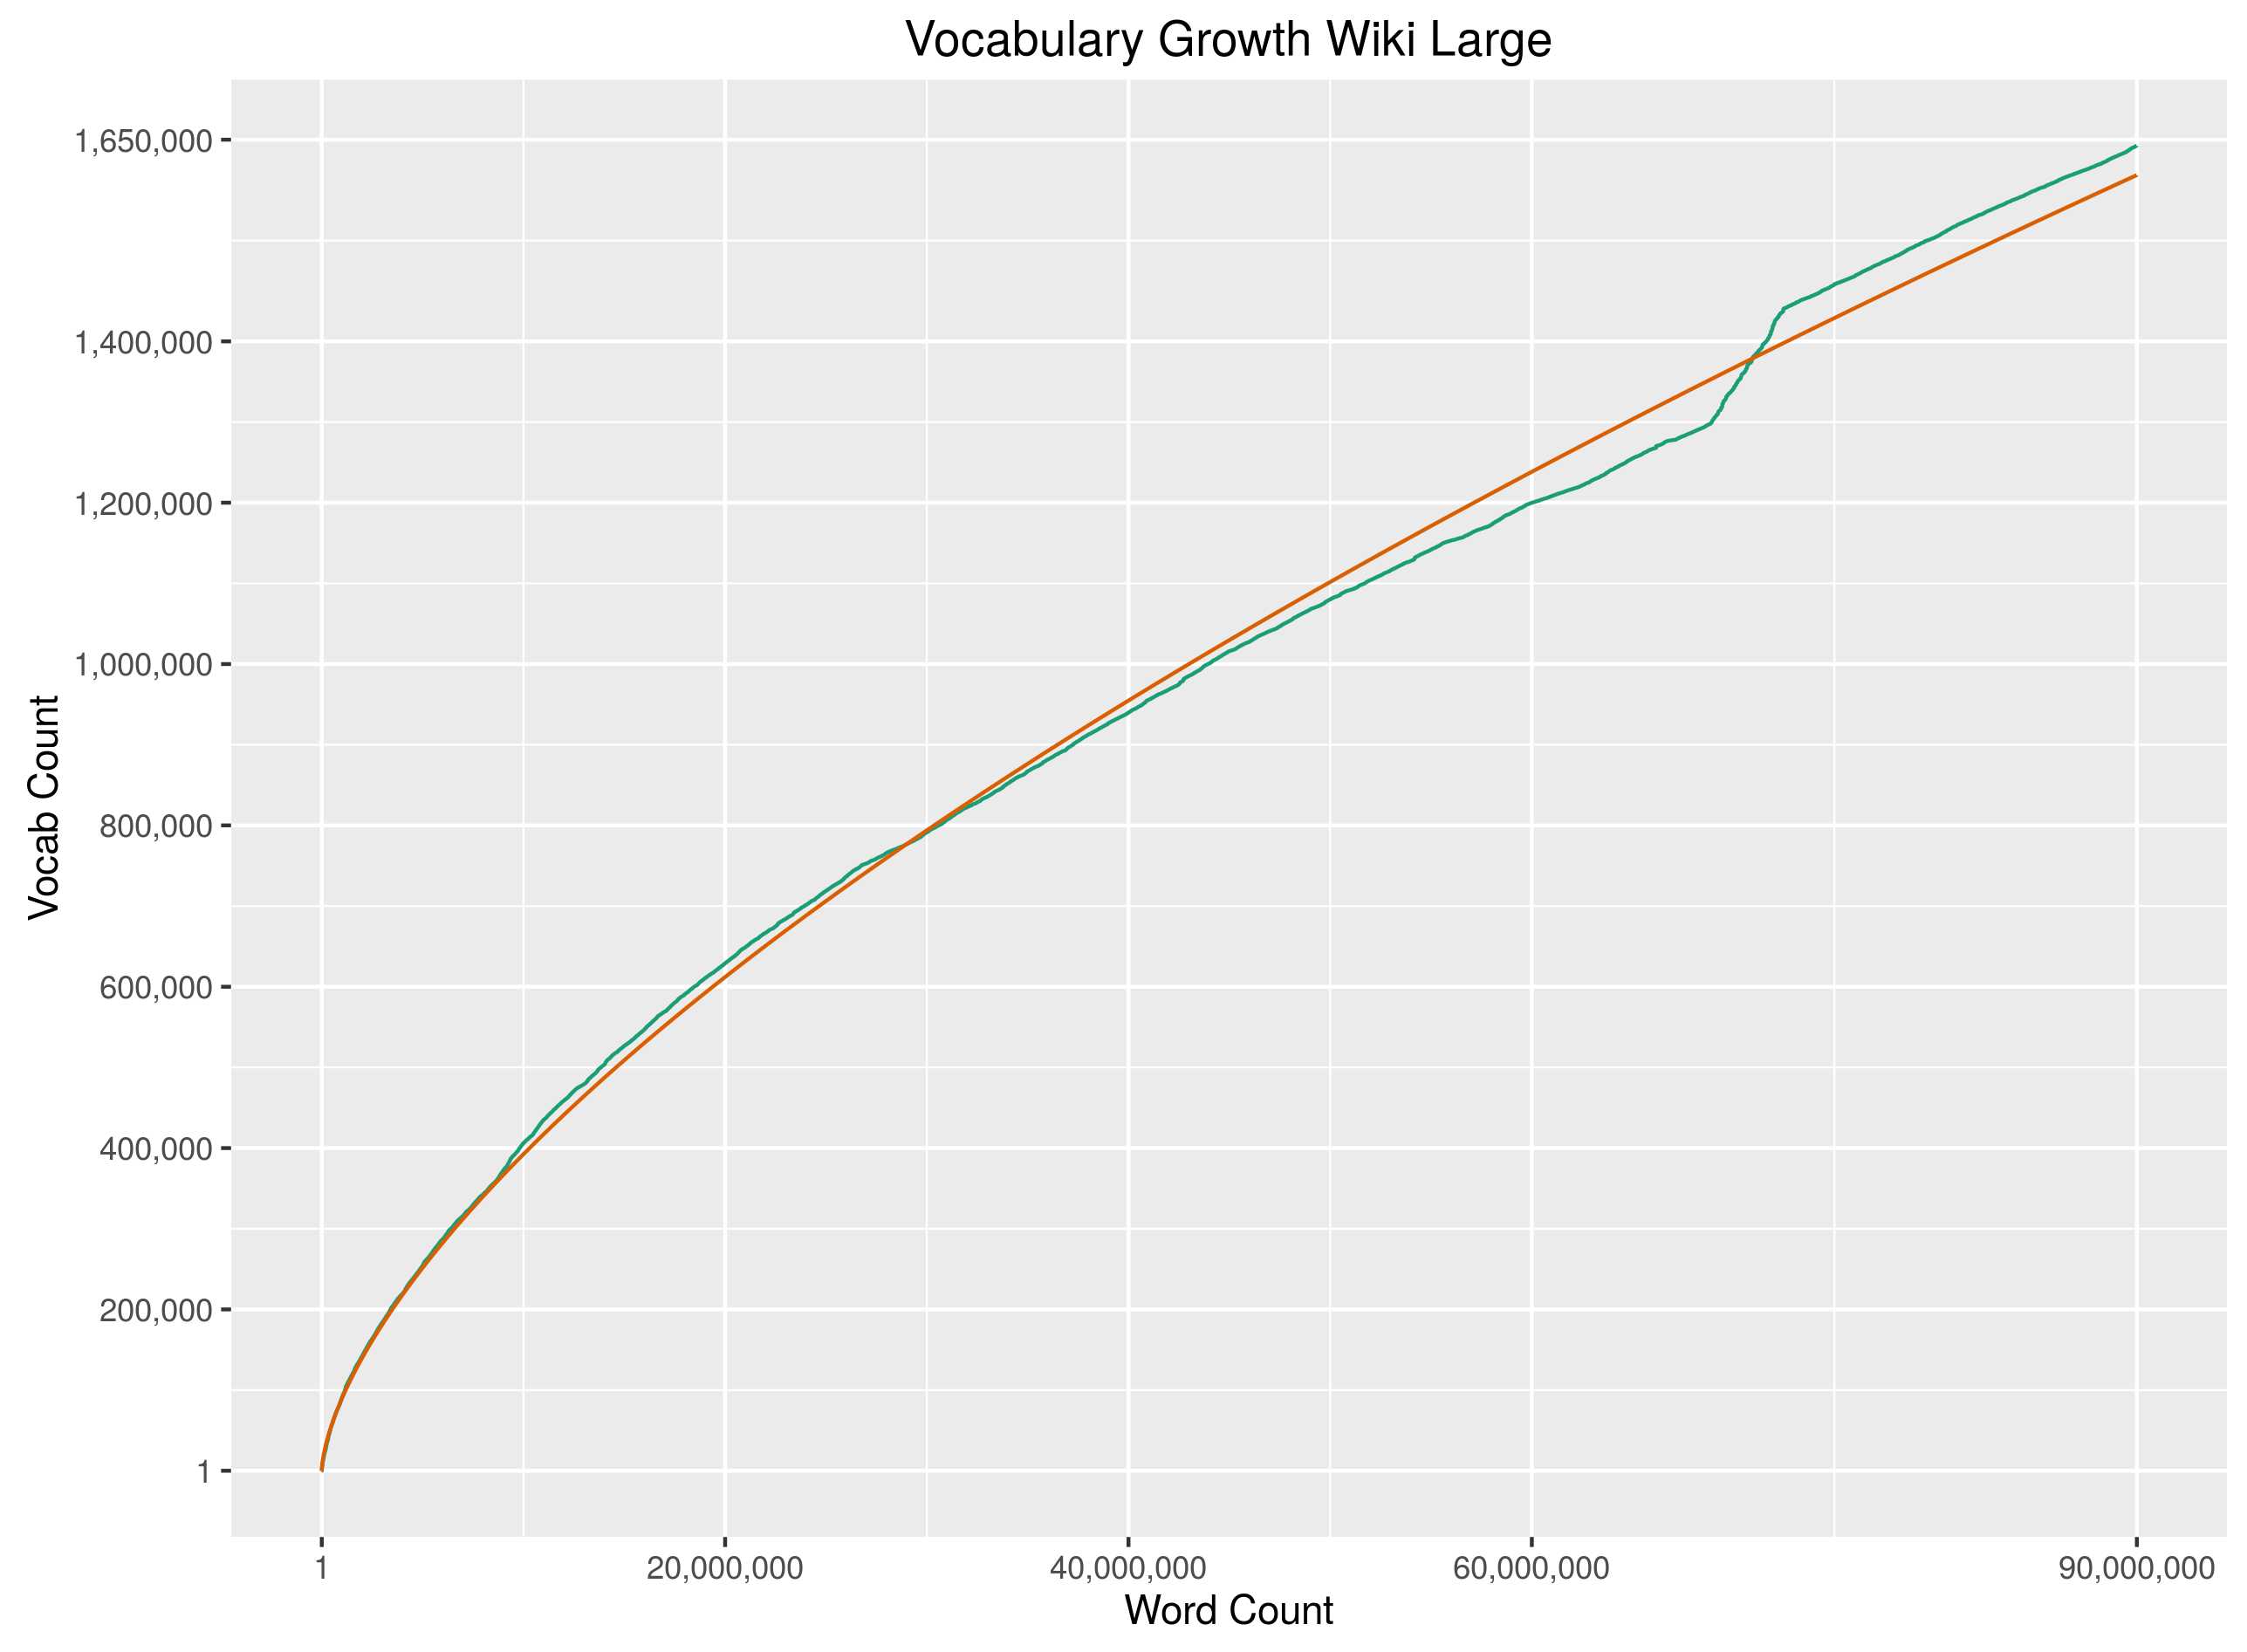
\includegraphics[scale=0.6]{wikiLargeVG.png}
\caption{Vocab Growth}
\label{fig:wvg}
\end{figure}

\noindent Processing the datasets in reverse order \autoref{fig:wvgr} shows the reverse of the in order processing but aligns closer to Heaps estimation. As state in the discussion for the in order processing the actual data shows that we incur the spike of new words at the beginning rather than at then where it now levels out.
\begin{figure}[H]
\centering
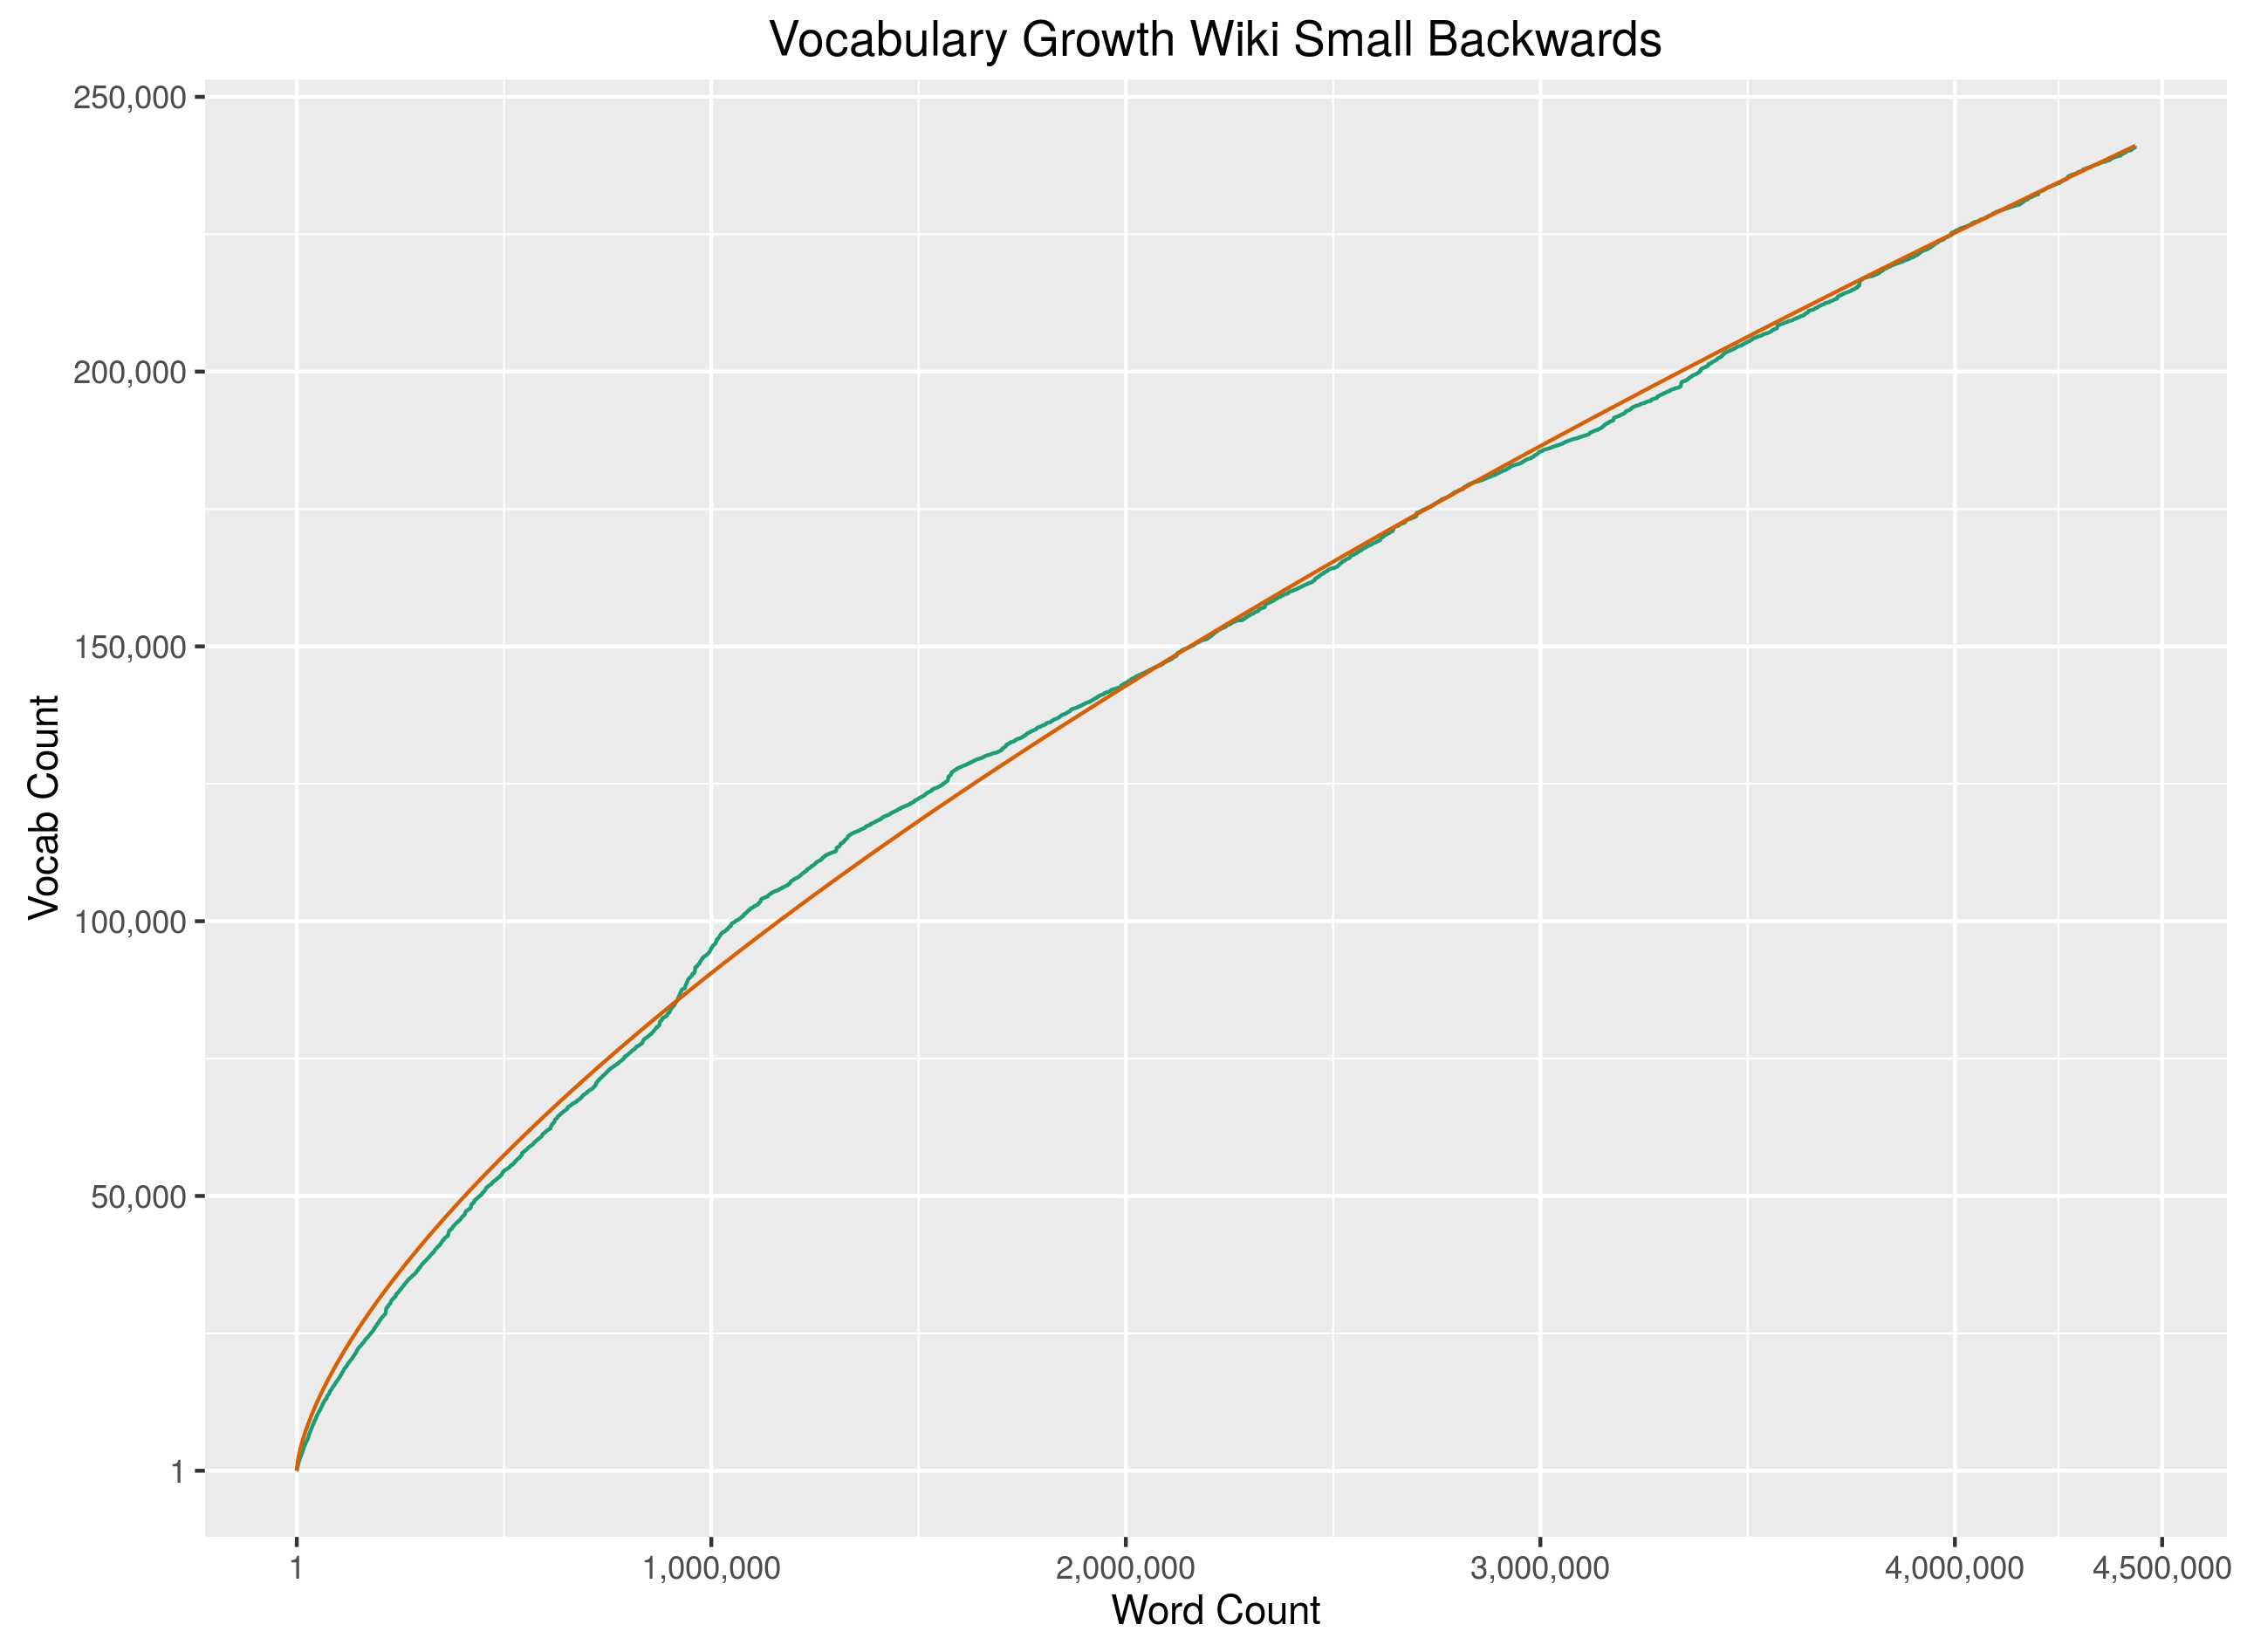
\includegraphics[scale=0.7]{wikiSmallVGB.png}
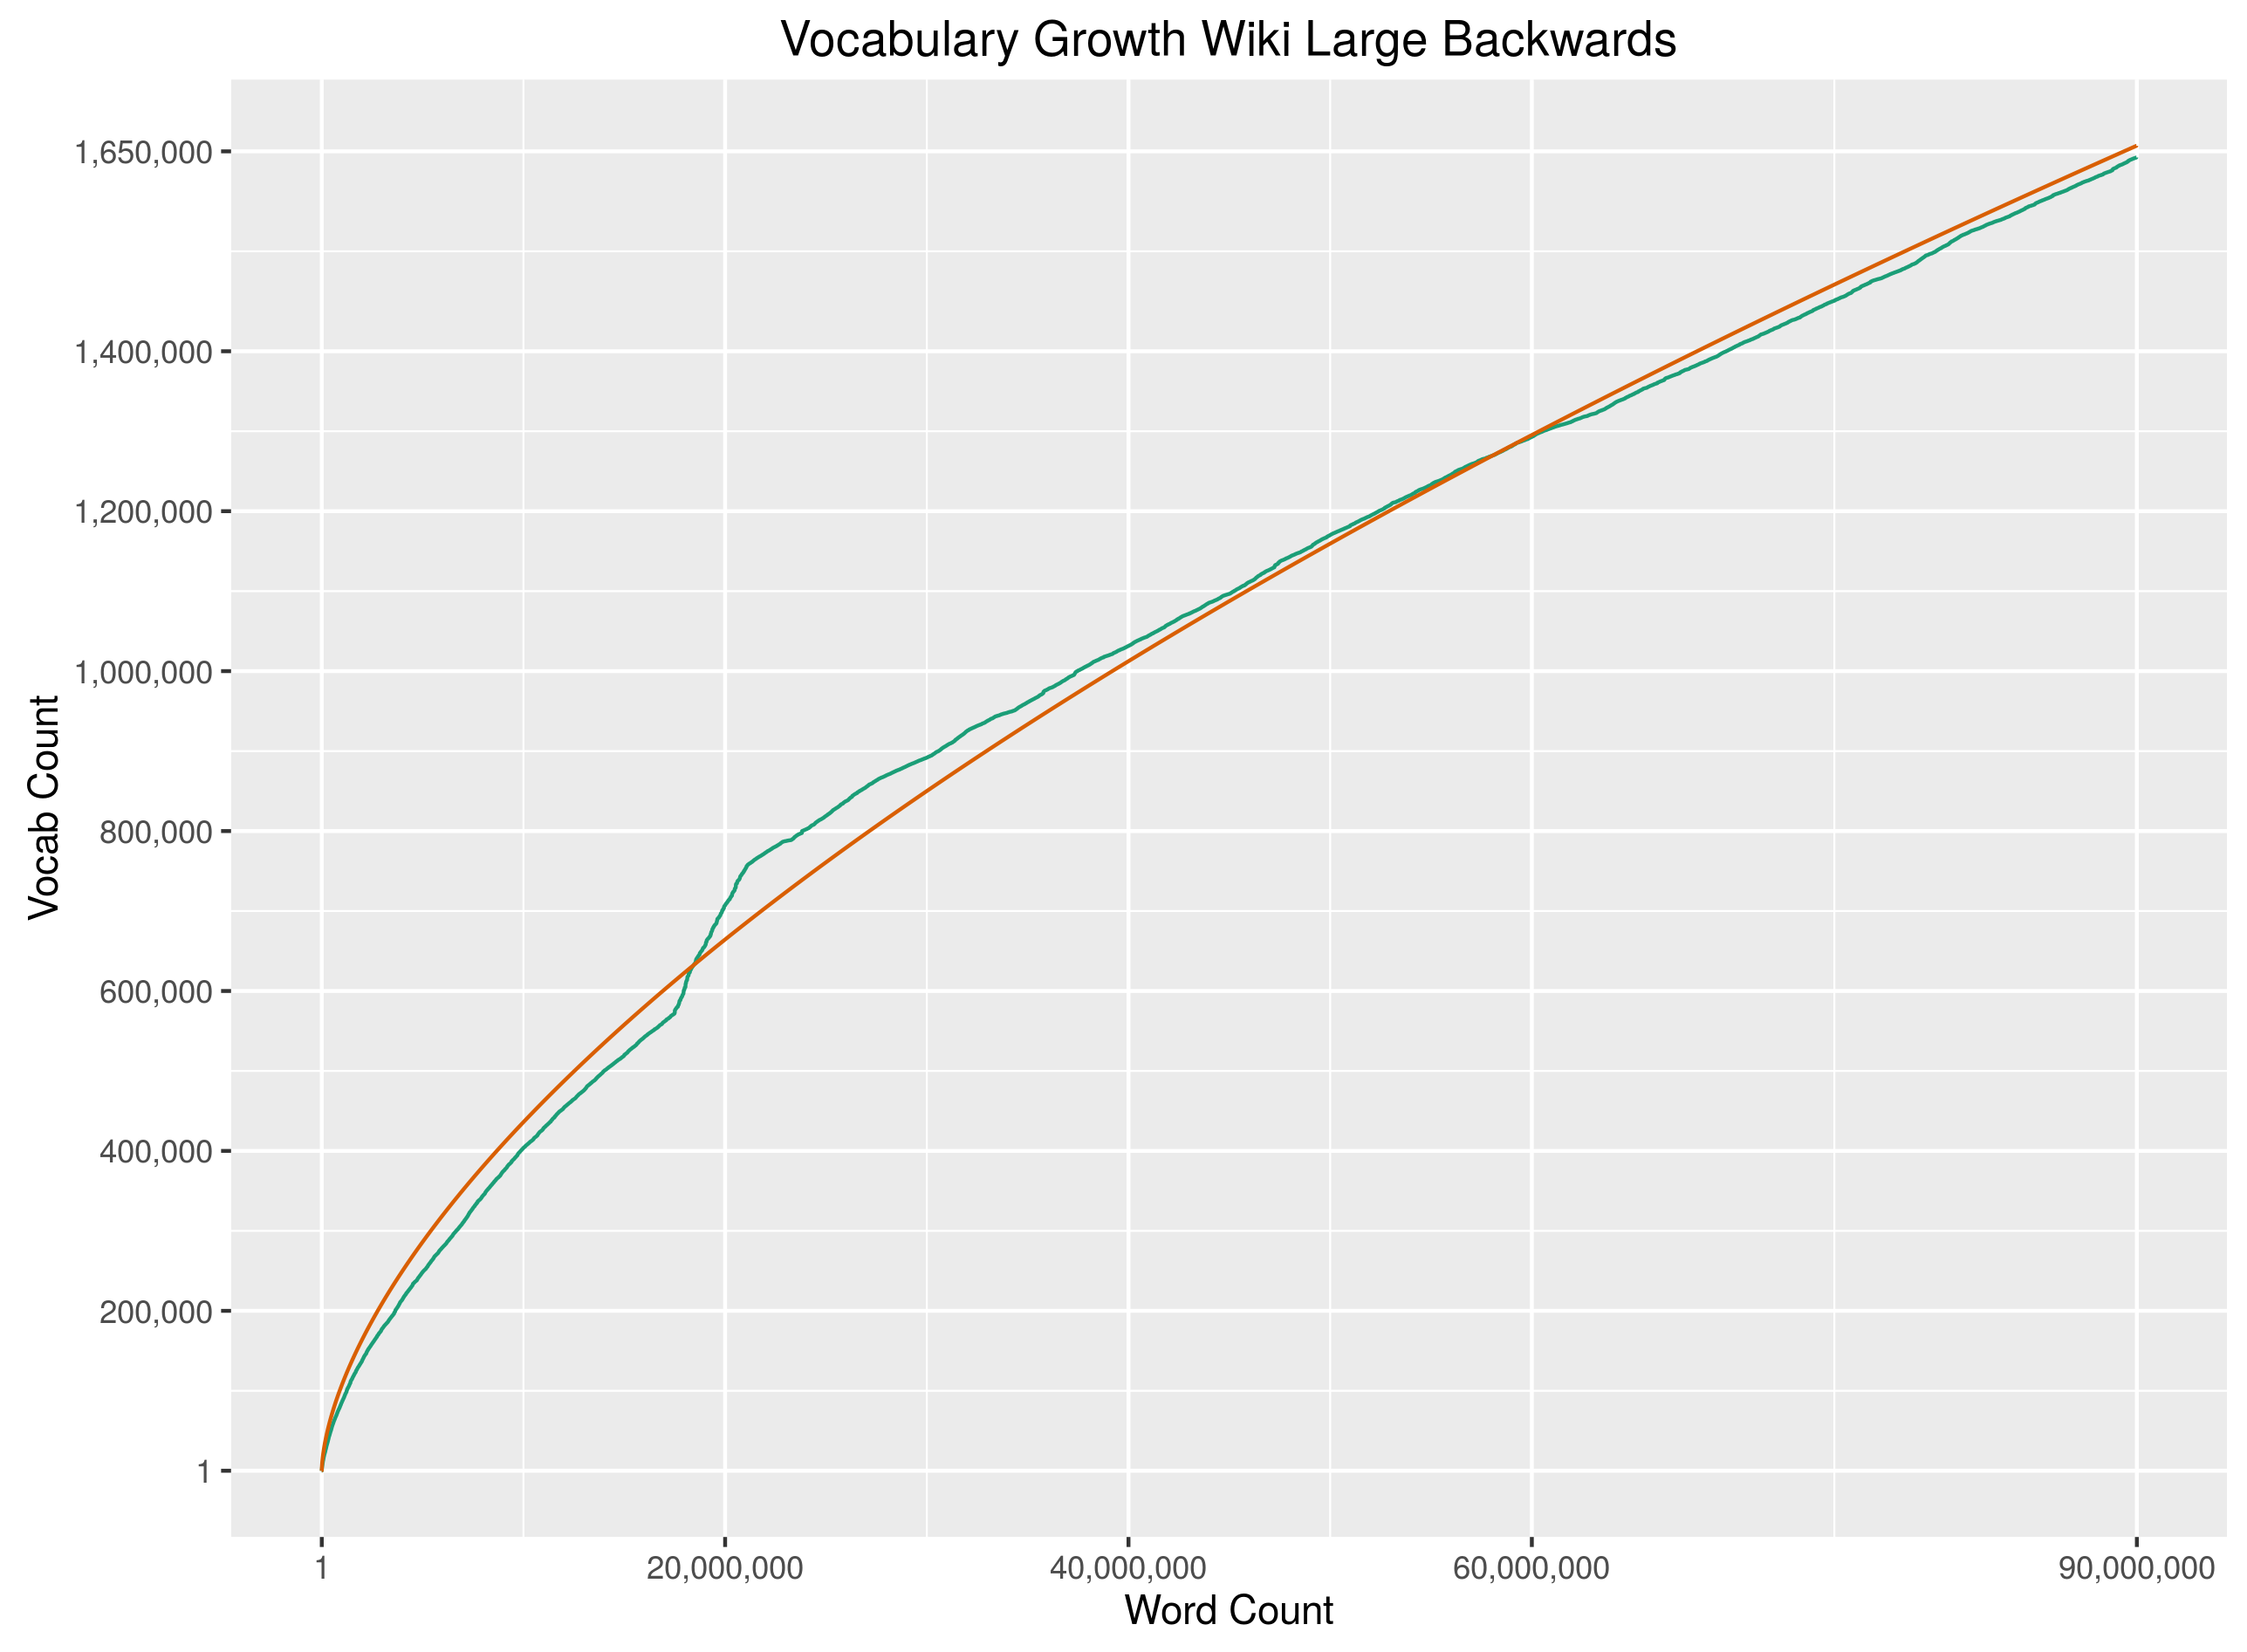
\includegraphics[scale=0.7]{wikiLargeVGB.png}
\caption{Vocab Growth Reverse Order}
\label{fig:wvgb}
\end{figure}
\noindent I choose to add the random order processing to this question as after plotting the dataset in order and reverse order as the plots caused me to wonder what its affect would be.
\autoref{fig:wvgr} shows that random selection for processing caused the actual data to be almost one to one with the estimate.   
\begin{figure}[H]
\centering
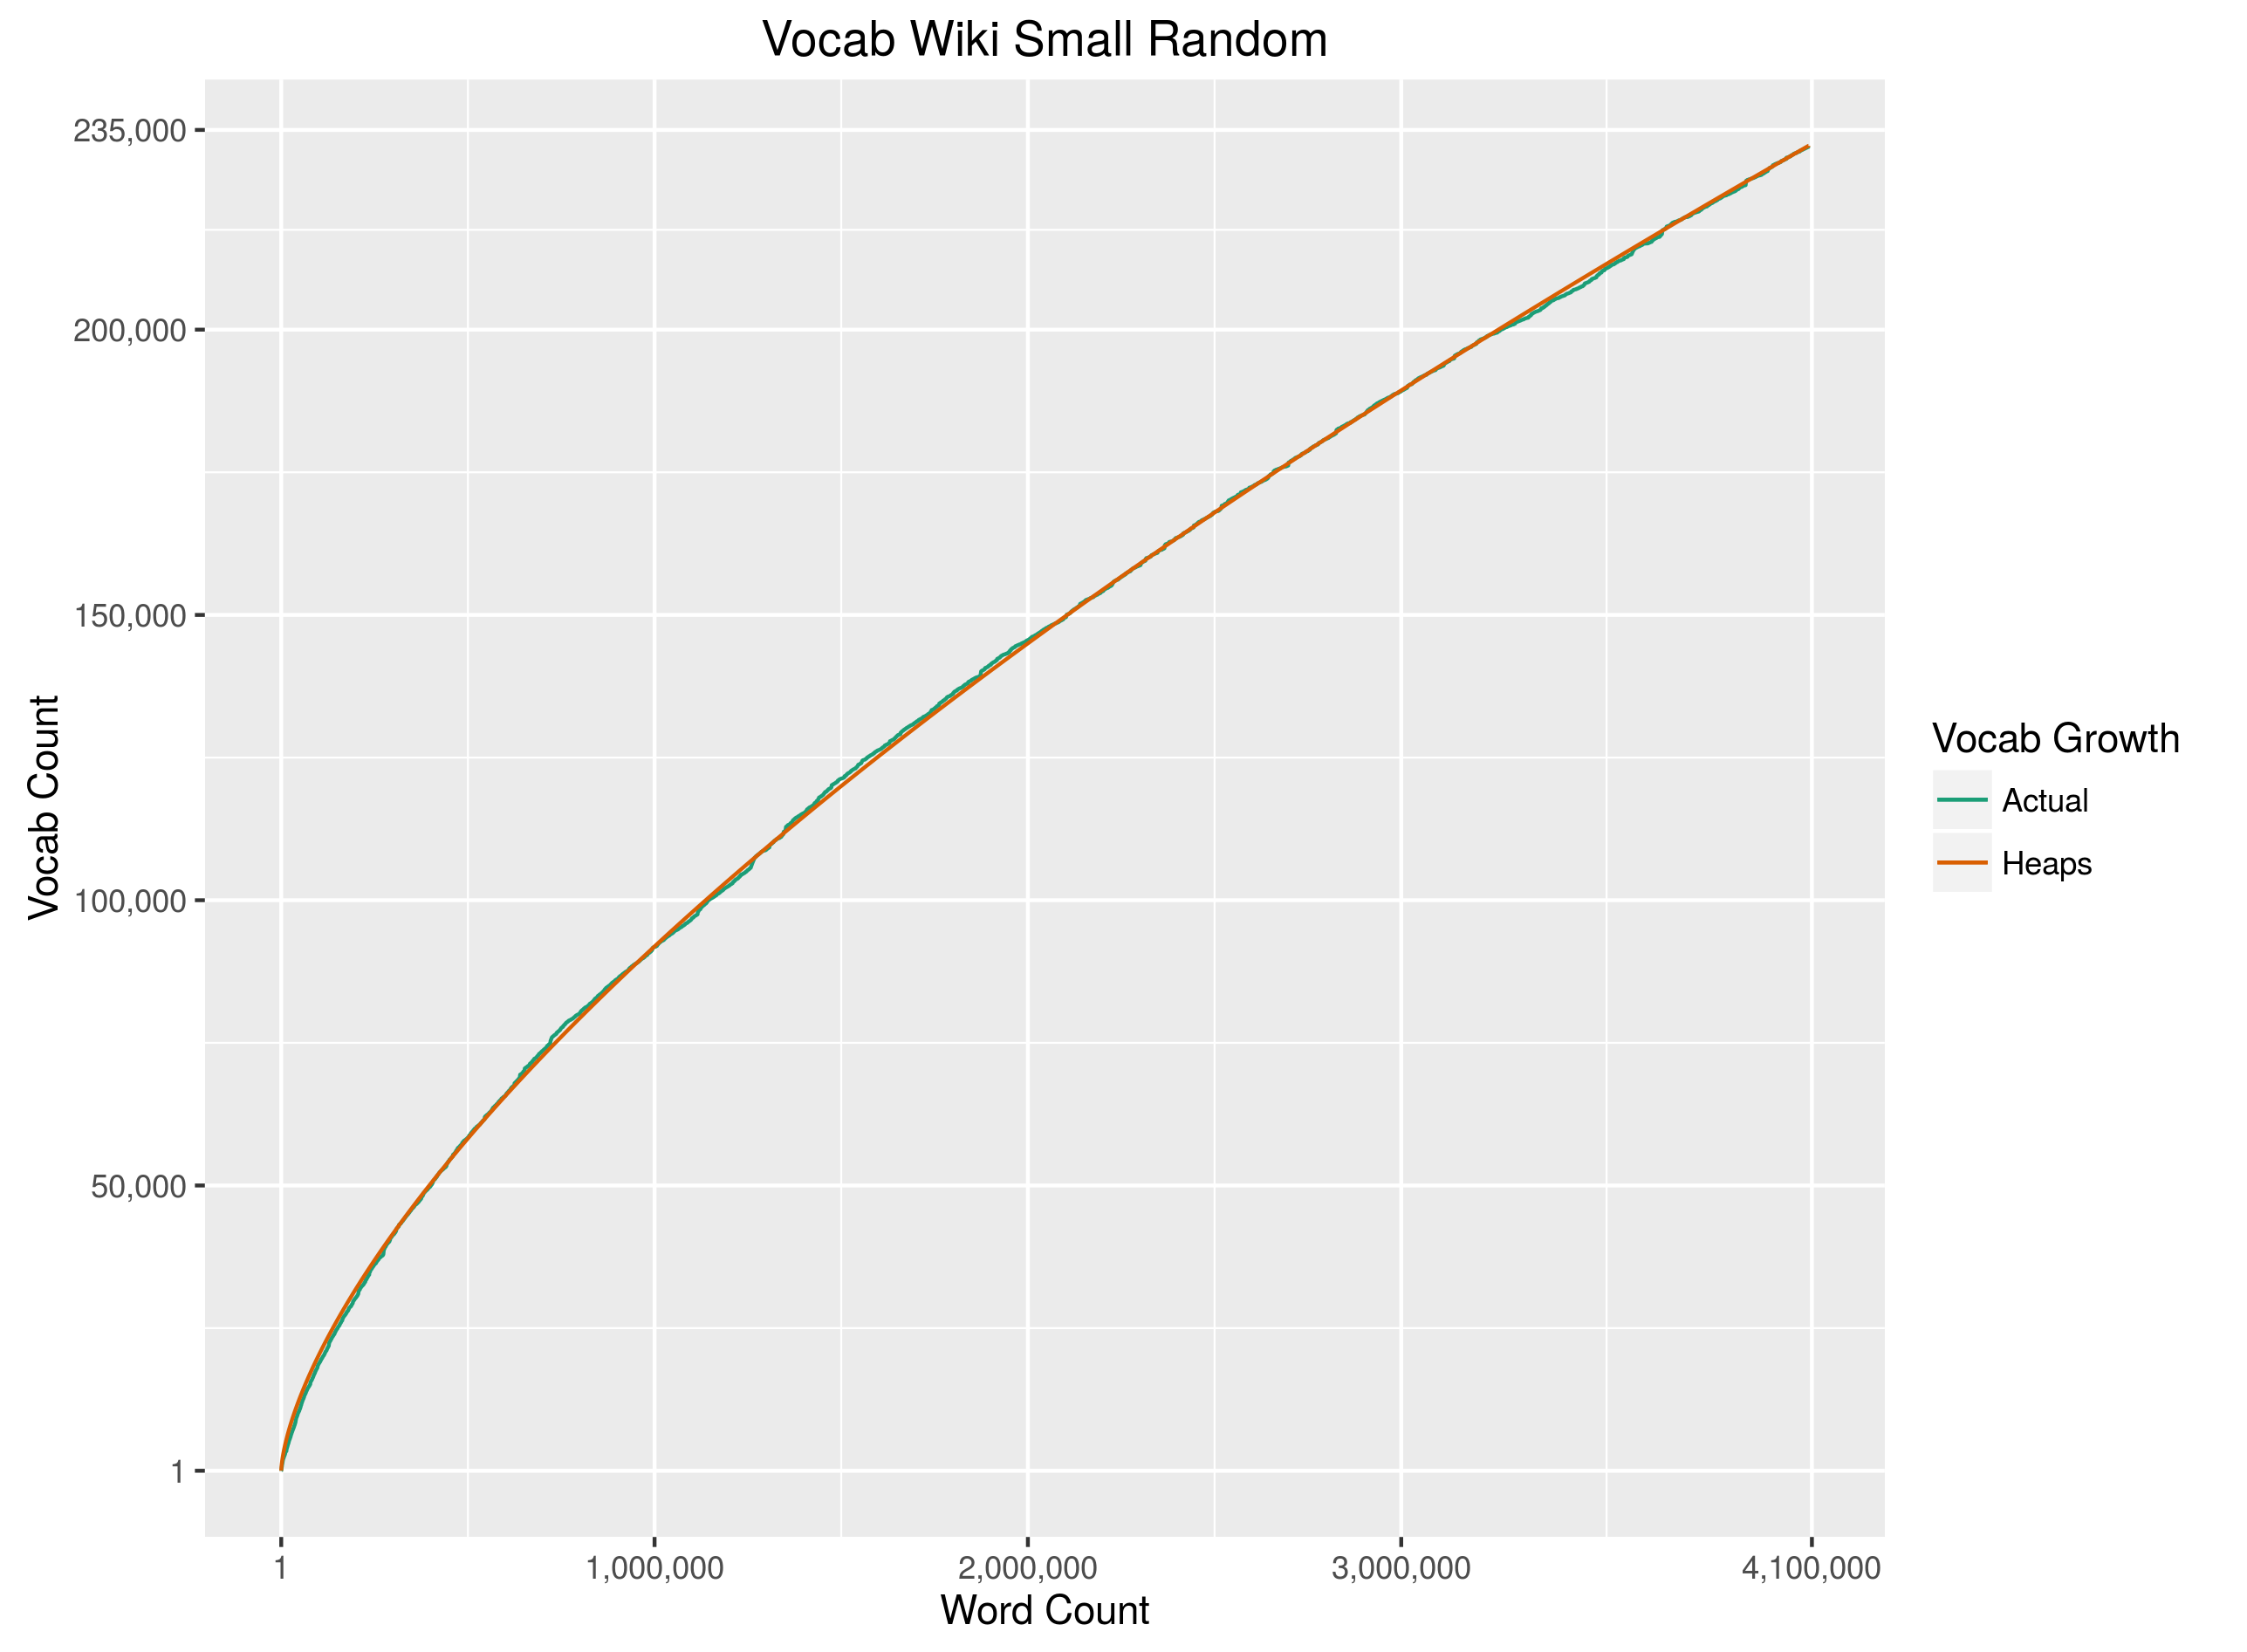
\includegraphics[scale=0.7]{wikiSmallVR.png}
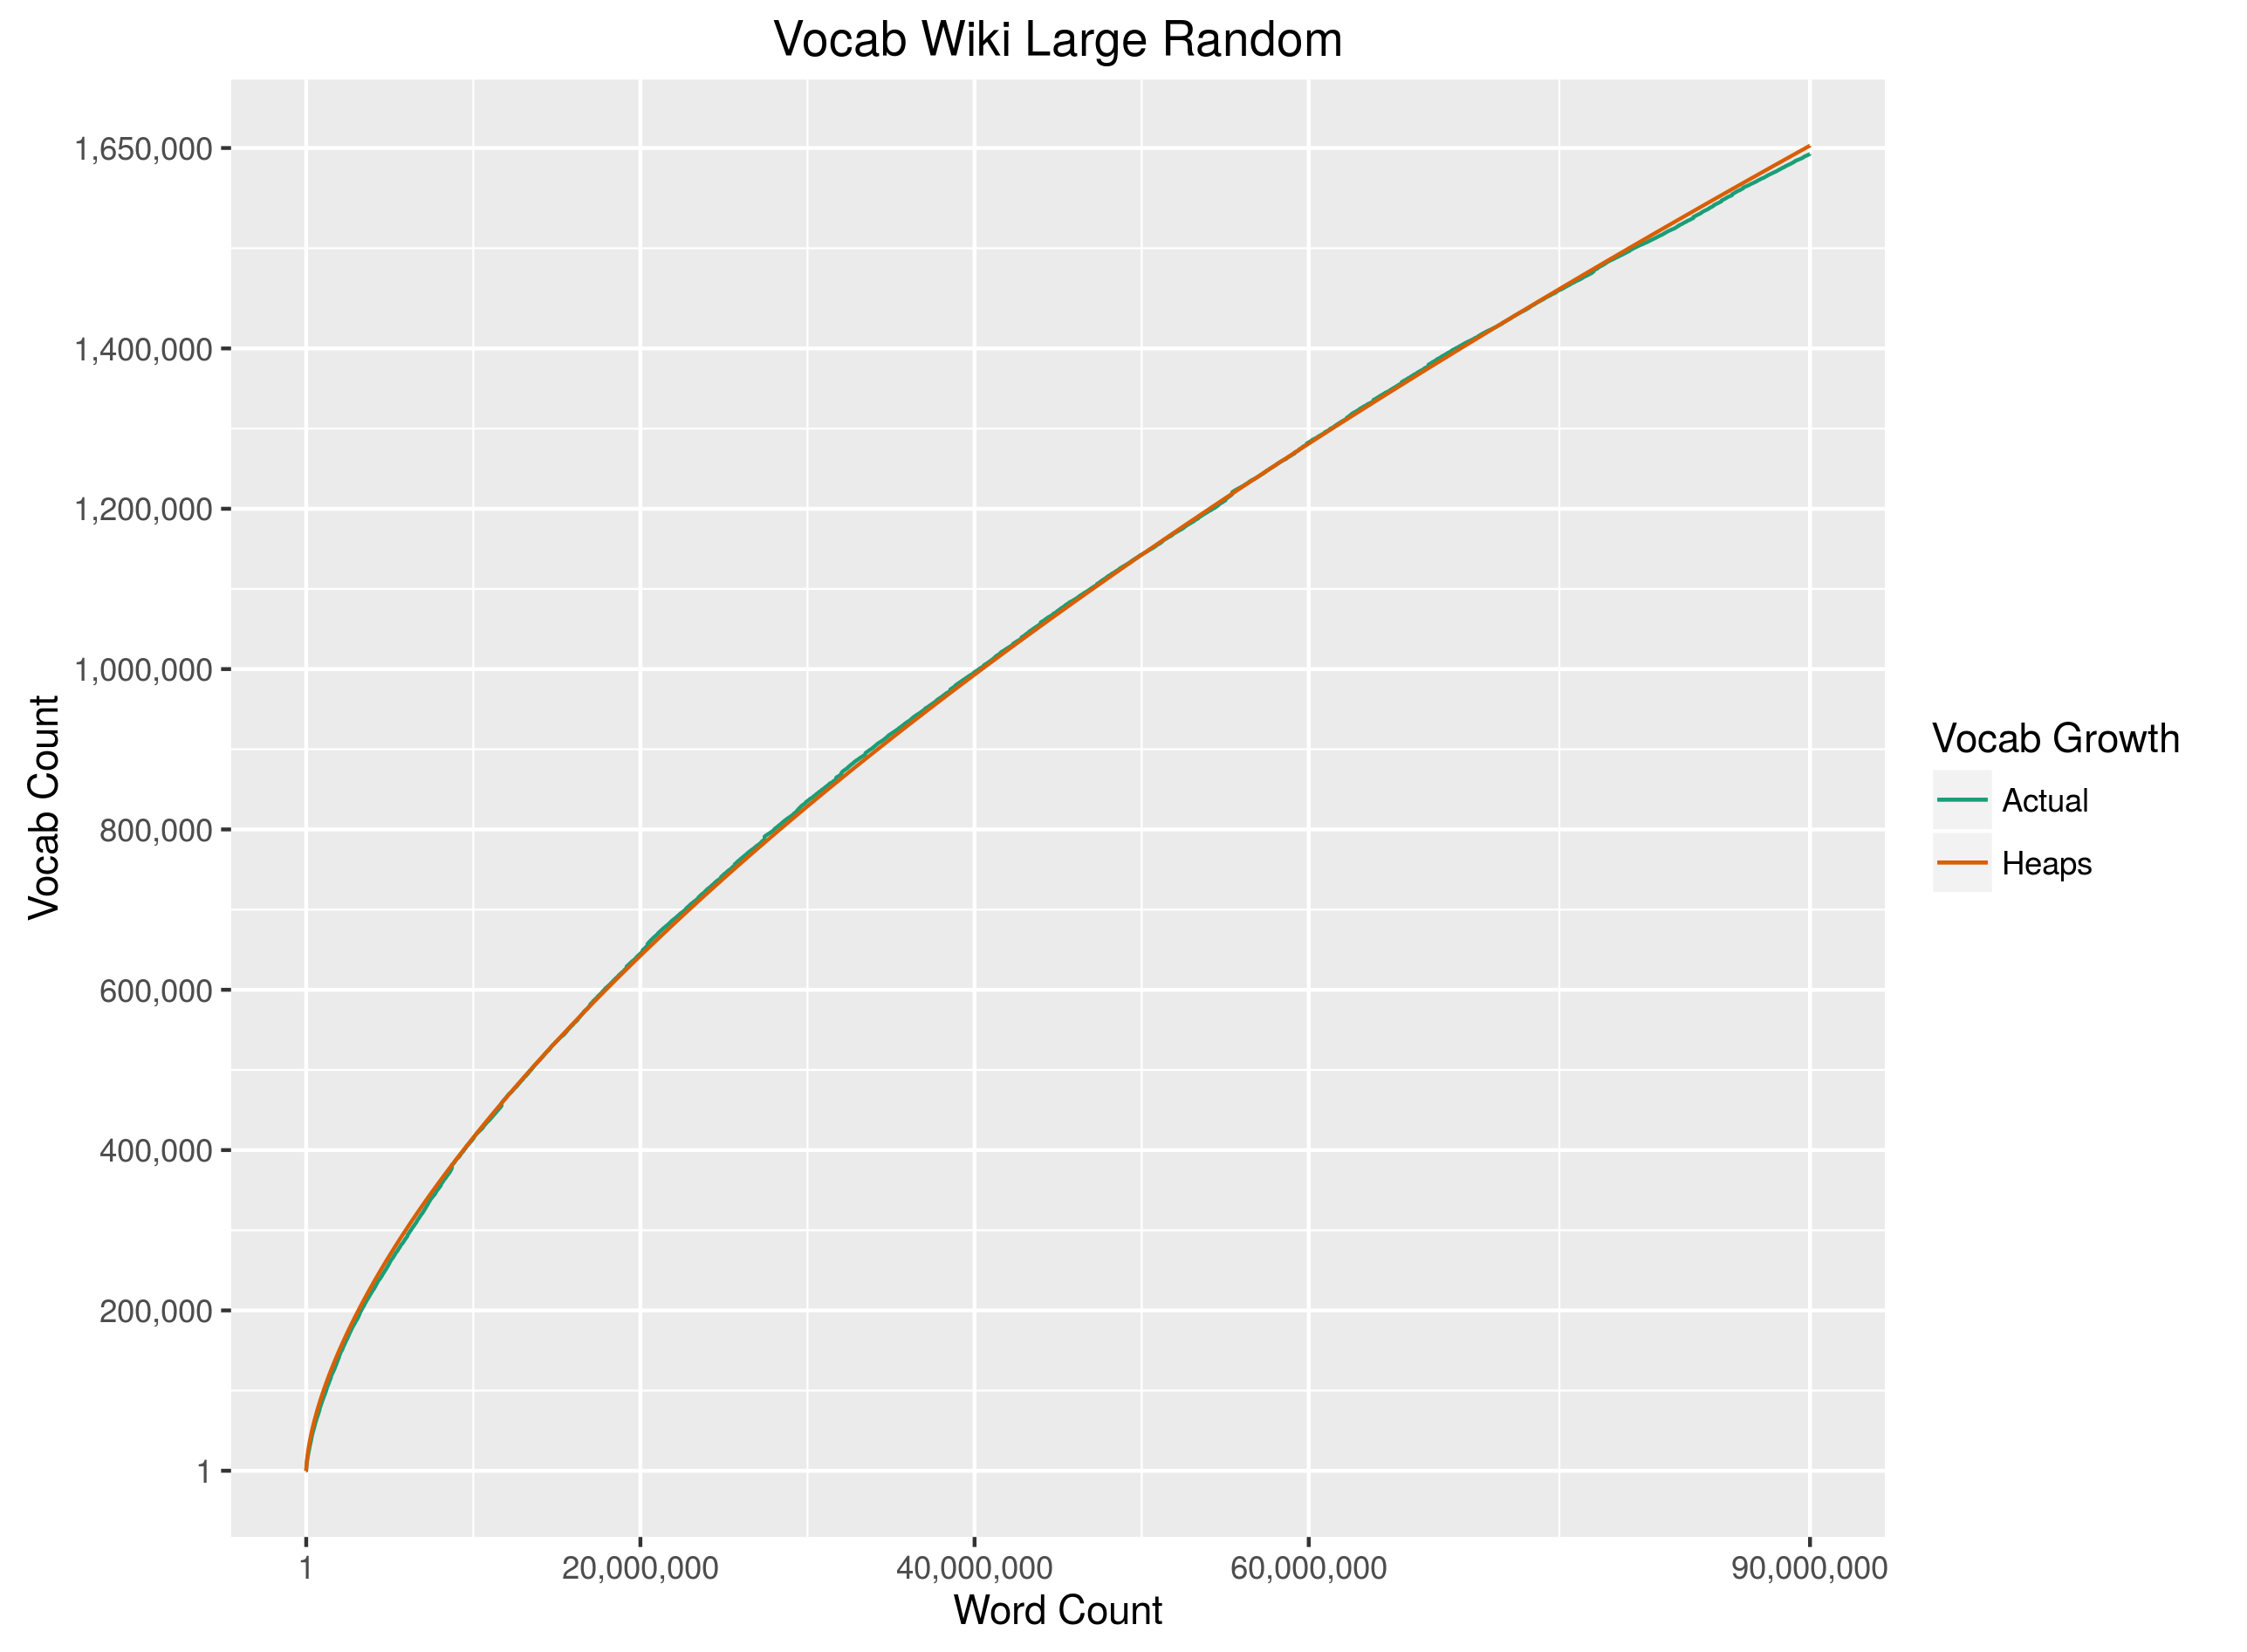
\includegraphics[scale=0.7]{wikiLargeVGR.png}
\caption{Vocab Growth Random Order}
\label{fig:wvgr}
\end{figure}
\noindent As shown in the plots for vocab processing, the order in which the they are seen does make a difference. The distribution of new words is primarily in the initial documents processed whereas more unique words are present towards the end of the documents. This was shown in  \autoref{fig:wvg} and \autoref{fig:wvgb} where reversing the order causes the fluctuation in new vocabulary words to happen at the beginning rather than at the end. Furthermore when processing the documents in random order \autoref{fig:wvgr} the distribution of new vocabulary entries to word count that would cause spikes in comparison to the estimation is negated. This negation, in our case with none English texts, shows that using Heaps estimation of vocabulary growth is an incredibly accurate irregardless of the mix of document languages in a dataset. \newline \newline  

\begin{code}
\captionof{listing}{Wiki Vocab Processing Code} \label{code:vcp}
	\pycode{code/wiki_vocab.py}
	
\end{code}
\begin{code}
\captionof{listing}{Wiki Vocab Plot Code} \label{code:vcr}
	\rcode{code/wiki-vocab.R}
	
\end{code}
\newpage
\section{Question 4.9}
\label{q:pr}
\begin{verbatim}
Compute PageRank for the Wikipedia documents. List the 20 documents
with the highest PageRank values together with the values.
\end{verbatim}
\subsection{Answer}
The computation of PageRank for both the small and large wiki sets was done using networkx a python ``graph" library. It has three methods for computing PageRank: pure python, using scipi and numpy. I choose the scipi method as it uses power iteration on a sparse matrix for the eigenvector calculation rather than simply iteration (pure python) or accessing LAPACKs eigenvalue solver via numpy (which threw errors due to size of the graph). Out links were determined using Beautiful soup to find all the a tags in an article that were relative to the location of the dataset using the regular expression \verb\'([.]{2}/){4}articles'\, filtering out image links and keeping out links that actually pointed to an article in the set. Two other variations were used called second and third. Both filtered out image links but the second only checked if the link was not a self link and the third used \verb\Soup.find_all('a', href=True)\ to find a tags with the other filtering methods from the first. It was found that some links use the $\sim$ character that pointed to pages not in the dataset but more times than not pointed to an actual page. To account for this the characters leftmost of the  $\sim$ and itself were removed leaving the actual pointed to page which was checked to see if it was in the dataset. The code for this process can be seen in \autoref{code:pr} and the sizes of the graph produces by each filtering method is seen in \autoref{tb:gs}.
\begin{table}[H]
\centering
\caption{Graph Sizes}
\label{tb:gs}
\begin{minipage}{.5\textwidth}
\begin{tabular}{llll}
Nodes & Edges & Method & Wiki Graph \\
6,043 & 608 & Filter 1 & Small \\
233,493 & 471,722 & Filter 2 & Small \\
233,493 & 471,722 & Filter 3 & Small \\
\end{tabular}
 \end{minipage}%
    \begin{minipage}{0.5\textwidth}
  \begin{tabular}{llll}
Nodes & Edges & Method & Wiki Graph \\
121,818 & 256,036 & Filter 1 & Large \\
1,763,461 & 9,549,718 & Filter 2 & Large \\
121,818 & 256,274 & Filter 3 & Large \\
\end{tabular}
\end{minipage}
\end{table}
\noindent The results of filtering method one for both the small and large Wiki dataset can be seen in \autoref{tb:wpr}. The ranks were not normalized as they show the raw data of the calculation given the sizes of the graphs. Method one for the small dataset produced a rather sparse graph whereas the large set produced a reasonable sized graph. The size of the small graph can only be attributed to the fact that in order to decrease the amount of articles included in the set while keeping some linkage between pages a wider variety had to used. The large graphs nodes UTC seemed odd to appear when using the first filtering method but indeed those pages do appear in the large dataset.\newline \newline \noindent
Filtering method 2 produced the largest graph for both the small and large set. \autoref{tb:wpr2}
shows the effect of keeping the extraneous links in the computation. Pages such as About, SmackBot, Bluebot are included and appear in both graphs. Both set graphs are the same except for the order in which the nodes appear.\newline \newline \noindent
Filtering method 3 produced the most interesting results seen in \autoref{tb:wpr3}. For the small set the number of nodes and edges remained the same from method 2 whereas the large sets edges increased by 38. What is also very interesting is the scores and pages are the same as was produced by method 1. The answer to why this happened may be found by considering the large sets graph. Its edges increase slightly leaving the PageRank results the same. This answer still leads me to believe human error for the small graph. 
\begin{table}[H]
\centering
\caption{Wiki Top 20 Page Rank}
\label{tb:wpr} 
\begin{minipage}{.5\textwidth}
\begin{tabular}{lc|}
\multicolumn{1}{c}{Wiki Small Page} & \multicolumn{1}{c|}{rank} \\
Brazil.html & 0.01739 \\
Fernando\_Collor\_de\_Mello\_1c42.html & 0.01497 \\
August\_26.html & 0.00963 \\
Kidney.html & 0.00620 \\
Diabetic\_nephropathy.html & 0.00537 \\
Seinfeld.html & 0.00201 \\
Ronald\_Colman\_8c1a.html & 0.00184 \\
Manga.html & 0.00172 \\
Magazine.html & 0.00166 \\
Broderick\_Crawford\_c49a.html & 0.00166 \\
1150.html & 0.00154 \\
Pope\_Innocent\_VIII\_650a.html & 0.00149 \\
Transjordan.html & 0.00147 \\
Gilbert\_and\_Ellice\_Islands\_8a4e.html & 0.00147 \\
Mollusca.html & 0.00145 \\
Pope\_Paul\_VI\_4529.html & 0.00143 \\
List\_of\_Navarrese\_monarchs\_334f.html & 0.00140 \\
F-102\_Delta\_Dagger\_058e.html & 0.00136 \\
Isthmian\_League\_1d48.html & 0.00136 \\
Pope\_Benedict\_IV\_b5de.html & 0.00135
\end{tabular}
 \end{minipage}%
    \begin{minipage}{0.5\textwidth}
    \begin{tabular}{lc}
\multicolumn{1}{c}{Wiki Large Page} & rank \\
Record\_label.html & 0.00855 \\
Music\_genre.html & 0.00812 \\
London.html & 0.00767 \\
UTC-5\_c184.html & 0.00551 \\
Brazil.html & 0.00498 \\
Radio.html & 0.00469 \\
UTC+2\_8d21.html & 0.00460 \\
Paris.html & 0.00460 \\
1966.html & 0.00383 \\
Romania.html & 0.00329 \\
The\_Byrds\_72ba.html & 0.00306 \\
1962.html & 0.00304 \\
1946.html & 0.00300 \\
July\_1.html & 0.00291 \\
UTC+7$\sim$30\_a9b0.html & 0.00282 \\
Herb\_Alpert\_5b74.html & 0.00281 \\
UTC+5\_6f4a.html & 0.00258 \\
UTC-10\_755d.html & 0.00255 \\
April\_15.html & 0.00251 \\
1930.html & 0.00240
\end{tabular}
\end{minipage}
\end{table}

\begin{table}[h]
\centering
\caption{Wiki Top 20 Page Rank Method 2}
\label{tb:wpr2} 
\begin{minipage}{.5\textwidth}
\begin{tabular}{lc|}
\multicolumn{1}{c}{Wiki Small Page} & \multicolumn{1}{c|}{rank} \\
Current\_events\_bb60.html & 0.00050 \\
RecentChanges\_e0d0.html & 0.00050 \\
Contact\_us\_afd6.html & 0.00050 \\
Community\_Portal\_6a3c.html & 0.00050 \\
About\_8d82.html & 0.00050 \\
Contents\_22de.html & 0.00050 \\
General\_disclaimer\_3e44.html & 0.00050 \\
Featured\_content\_5442.html & 0.00050 \\
Contents\_b878.html & 0.00050 \\
Categories\_101d.html & 0.00049 \\
Stub\_72af.html & 0.00017 \\
SmackBot\_cc7a.html & 0.00012 \\
Find\_or\_fix\_a\_stub\_e7c5.html & 0.00010 \\
Perfect\_stub\_article\_2d8f.html & 0.00009 \\
Alaibot\_de3d.html & 0.00007 \\
Disambiguation\_78fc.html & 0.00005 \\
United\_States\_09d4.html & 0.00005 \\
Living\_people\_7259.html & 0.00005 \\
Bluebot\_e595.html & 0.00004 \\
Geographic\_coordinate\_system.html & 0.00004
\end{tabular}
 \end{minipage}%
    \begin{minipage}{0.5\textwidth}
    \begin{tabular}{lc}
\multicolumn{1}{c}{Wiki Large Page} & rank \\
Current\_events\_bb60.html & 0.00130 \\
Community\_Portal\_6a3c.html & 0.00130 \\
Contact\_us\_afd6.html & 0.00130 \\
RecentChanges\_e0d0.html & 0.00130 \\
General\_disclaimer\_3e44.html & 0.00130 \\
Featured\_content\_5442.html & 0.00130 \\
About\_8d82.html & 0.00130 \\
Contents\_22de.html & 0.00130 \\
Contents\_b878.html & 0.00130 \\
Categories\_101d.html & 0.00129 \\
Stub\_72af.html & 0.00044 \\
SmackBot\_cc7a.html & 0.00032 \\
Find\_or\_fix\_a\_stub\_e7c5.html & 0.00024 \\
Perfect\_stub\_article\_2d8f.html & 0.00023 \\
Alaibot\_de3d.html & 0.00019 \\
United\_States\_09d4.html & 0.00013 \\
Living\_people\_7259.html & 0.00013 \\
Disambiguation\_78fc.html & 0.00013 \\
Bluebot\_e595.html & 0.00011 \\
Geographic\_coordinate\_system.html & 0.00011
\end{tabular}
\end{minipage}
\end{table}

\begin{table}[h]
\centering
\caption{Wiki Top 20 Page Rank Method 3}
\label{tb:wpr3} 
\begin{minipage}{.5\textwidth}
\begin{tabular}{lc|}
\multicolumn{1}{c}{Wiki Small Page} & \multicolumn{1}{c|}{rank} \\
Brazil.html & 0.01739 \\
Fernando\_Collor\_de\_Mello\_1c42.html & 0.01497 \\
August\_26.html & 0.00963 \\
Kidney.html & 0.00620 \\
Diabetic\_nephropathy.html & 0.00537 \\
Seinfeld.html & 0.00201 \\
Ronald\_Colman\_8c1a.html & 0.00184 \\
Manga.html & 0.00172 \\
Magazine.html & 0.00166 \\
Broderick\_Crawford\_c49a.html & 0.00166 \\
1150.html & 0.00154 \\
Pope\_Innocent\_VIII\_650a.html & 0.00149 \\
Transjordan.html & 0.00147 \\
Gilbert\_and\_Ellice\_Islands\_8a4e.html & 0.00147 \\
Mollusca.html & 0.00145 \\
Pope\_Paul\_VI\_4529.html & 0.00143 \\
List\_of\_Navarrese\_monarchs\_334f.html & 0.00140 \\
F-102\_Delta\_Dagger\_058e.html & 0.00136 \\
Isthmian\_League\_1d48.html & 0.00136 \\
Pope\_Benedict\_IV\_b5de.html & 0.00135
\end{tabular}
 \end{minipage}%
    \begin{minipage}{0.5\textwidth}
    \begin{tabular}{lc}
\multicolumn{1}{c}{Wiki Large Page} & rank \\
Record\_label.html & 0.00855 \\
Music\_genre.html & 0.00812 \\
London.html & 0.00766 \\
UTC-5\_c184.html & 0.00550 \\
Brazil.html & 0.00495 \\
Radio.html & 0.00467 \\
Paris.html & 0.00459 \\
UTC+2\_8d21.html & 0.00459 \\
1966.html & 0.00387 \\
Romania.html & 0.00327 \\
The\_Byrds\_72ba.html & 0.00306 \\
1962.html & 0.00303 \\
1946.html & 0.00300 \\
July\_1.html & 0.00291 \\
UTC+7$\sim$30\_a9b0.html & 0.00281 \\
Herb\_Alpert\_5b74.html & 0.00281 \\
UTC+5\_6f4a.html & 0.00258 \\
UTC-10\_755d.html & 0.00254 \\
April\_15.html & 0.00252 \\
1930.html & 0.00240
\end{tabular}
\end{minipage}
\end{table}
\newpage
\clearpage
\begin{code}
	\pycode{code/wiki_pagerank.py}
	\captionof{listing}{Wiki PageRank Code} \label{code:pr}
\end{code}

\newpage
\section{Question 4.8}
\begin{verbatim}
Find the 10 Wikipedia documents with the most inlinks. Show the collec-
tion of anchor text for those pages
\end{verbatim}
\subsection{Answer}
I used the graphs generated from filtering method one used in the answer to Q2 question 4.9. 
As seen in \autoref{tb:wil} the inlinks for the small set is much smaller in comparison to the large set. Due the vast size differences the counts for the number of anchor texts is shown and the full anchor texts is include in the output\_files directory. The graphs were read in from the pickled format and in links for were gotten and sorted based on the length. The sorted list took the top ten and for each of the ten BeautifulSoup was used to extract the anchor text for all the links as seen in \autoref{code:wil}. \newline \newline \noindent
I will show a small section of the anchor texts for the top pages as a complete listing would not be presentable. \newline

\begin{minipage}{.5\textwidth}
\begin{verbatim}
Brazil.html
Brazil (disambiguation) 
Flag 
Coat of arms 
Motto 
Anthem 
Hino Nacional Brasileiro 
National seal 
Selo Nacional do Brasil 
Capital 
Brasília 
Largest city 
São Paulo
\end{verbatim}
 \end{minipage}
    \begin{minipage}{0.5\textwidth}
\begin{verbatim}
Music_genre.html
Electronic art music
Experimental music
Minimalist music
Jazz
Popular music
Traditional music
Folk music
Oral transmission
List of music genres
Art music
European classical music
List of classical music styles
\end{verbatim}
\end{minipage}

\begin{table}[H]
\centering
\caption{Wiki Top 10 In Links}
\label{tb:wil} 
\begin{tabular}{lc|}
\multicolumn{1}{c}{Wiki Small Page} & \multicolumn{1}{c}{Anchor Text Count}\\
Brazil.html & 87 \\
August\_26.html & 25 \\
Manga.html & 14 \\
Magazine.html & 13 \\
Mollusca.html & 12 \\
Screenwriter.html & 8 \\
Victoria\_of\_the\_United\_Kingdom\_5e8e.html & 8 \\
Kidney.html & 6 \\
Tottenham\_Hotspur\_F.C.\_6bd2.html & 5 \\
Tuscany.html & 4  
\end{tabular}
    \begin{tabular}{lc}
\multicolumn{1}{c}{Wiki Large Page} & Anchor Text Count\\
Music\_genre.html  & 6030  \\
Record\_label.html & 5844  \\
London.html        & 2903  \\
UTC-5\_c184.html   & 1543  \\
Brazil.html        & 1535  \\
Paris.html         & 1516  \\
UTC+2\_8d21.html   & 1319  \\
Romania.html       & 1198  \\
1966.html          & 1188  \\
1962.html          & 1127 
\end{tabular}
\end{table}
\newpage
\begin{code}
	\pycode{code/wiki-inlinks.py}
	\captionof{listing}{Wiki Inlink Code} \label{code:wil}
\end{code}
\newpage
\section{Question 5.8}
\begin{verbatim}
Write a program that can build a simple inverted index of a set of text docu-
ments. Each inverted list will contain the file names of the documents that contain
that word. (Dr. Nelson: use examples from the Wikipedia data set) 
\end{verbatim}
\subsection{Answer}
As mentioned at the beginning of this report the size of the inverted index for the large set prohibits it from being included with this report and it follows the full contents would not be shown. The same goes for the small set but its file is included with this report as its size is only a mere 61.5mb. The size factor came into play as my initial implementation built the inverted index in memory using pythons defaultdict backed by a set. The initial implementation worked well for the small set but when I applied it to the large set, I found after letting it run for 45min+, that it used 11gb of memory and in combination with Chrome was about to cause kernel panic due to the swap space for Linux being used up entirely. Yes kernel panic due to memory consumption, I have had it happen before and it was not fun at all. To fix this issue the file and a single word were written to a file as they appeared and then was read from to build the inverted index. This brought down the memory usage for the large set to about 9gb. The tokenization method used for the  Wiki vocabulary question was used here and the full code can be seen in \autoref{code:iidx}.
\autoref{tb:wii} shows the top 20 words and the number of documents found in.
\begin{table}[H]
\centering
\caption{Wiki Inverted Index}
\label{tb:wii} 
\begin{tabular}{ll|}
Wiki Small Word & Number Of Article Found In \\
wikimedia & 6043 \\
articlediscussioncurrent & 6043 \\
nonprofit & 6043 \\
gnu & 6043 \\
contents & 6043 \\
help & 6043 \\
if & 6043 \\
wikipedia® & 6043 \\
ismsie55 & 6043 \\
gen & 6043 \\
revision & 6043 \\
disclaimers & 6043 \\
changes & 6043 \\
search & 6043 \\
text & 6043 \\
trademark & 6043 \\
registered & 6043 \\
encyclopedia & 6043 \\
of & 6043 \\
inc & 6043
\end{tabular}
 \begin{tabular}{ll}
Wiki Large Word & Number Of Article Found In \\
to & 121818 \\
by & 121816 \\
revision & 121816 \\
last & 121816 \\
wikipedia® & 121816 \\
foundation & 121816 \\
7emonobook & 121816 \\
of & 121816 \\
skins & 121816 \\
under & 121816 \\
registered & 121816 \\
s & 121816 \\
wikimedia & 121816 \\
terms & 121816 \\
7ecommon & 121816 \\
contents & 121816 \\
featured & 121816 \\
this & 121816 \\
gen & 121816 \\
encyclopedia & 121816
\end{tabular}
\end{table}
\newpage
\begin{code}
	\pycode{code/wikis_inverted_idx.py}
	\captionof{listing}{Wiki Inverted Index Code} \label{code:iidx}
\end{code}
\newpage
\section{Question 5.14}
\begin{verbatim}
In section 5.7.3, we saw that the optimal skip distance c can be determined
by minimizing the quantity kn/c + pc/2, where k is the skip pointer length, n
is the total inverted list size, c is the skip interval, and p is the number of postings
to find.
Plot this function using k = 4, n = 1,000,000, and p = 1,000, but varying c.
Then, plot the same function, but set p = 10,000. Notice how the optimal value
for c changes.
Finally, take the derivative of the function kn/c + pc/2 in terms of c to find
the optimum value for c for a given set of other parameters (k, n, and p).
\end{verbatim}
\subsection{Answer}
\autoref{fig:skbp} shows the plot for both p=1,000 and p=10,000. Please note that this plot has had as small amount of jitter applied to the points as both functions start out the same but diverge from each other quickly. This is due to the starting point for the function which is zero. The lower p value cause the function to grow rather slowly where as the large p value combined with the same c value the function grows faster. \newline \newline The first derivative of the skip distance function in terms of c is $\displaystyle \frac{p}{2}  - \frac{k n}{c ^{2}}$ and was generated using the R code seen in \autoref{code:dsd}. Finding the optimal c value for the function with p=1,000 and p=10,000 required me to do some thinking. After some thought I recalled what I had learned in the cs undergraduate numerical methods class here at ODU for root approximation of a function. The root approximation methods found the zeros of a function within a tolerance and the number which gave the zero is considered the functions root. This is much like what we want for this question. So I went looking for what would do this in R and discovered the grad function from the numDeriv package and from the documentation ``The function grad calculates a numerical approximation of the first derivative of func at the point x". Using the grad function I generated the functions return values for a given c. The c values used for the two functions differ as after plotting various c values I found that for p=1,000 the c values from 10 to 200 showed the best results and for p=10,000 c values from 10:100.  The optimal c value for the two functions was found by taking the maximum corresponding value whose approximation value was closest to or equal to zero. \autoref{fig:skdp} shows the plot for p=1,000 which had an optimal c value of 89 and \autoref{fig:skdp2} shows the plot for p=10,000 which had an optimal c value of 28.
\begin{figure}[h]
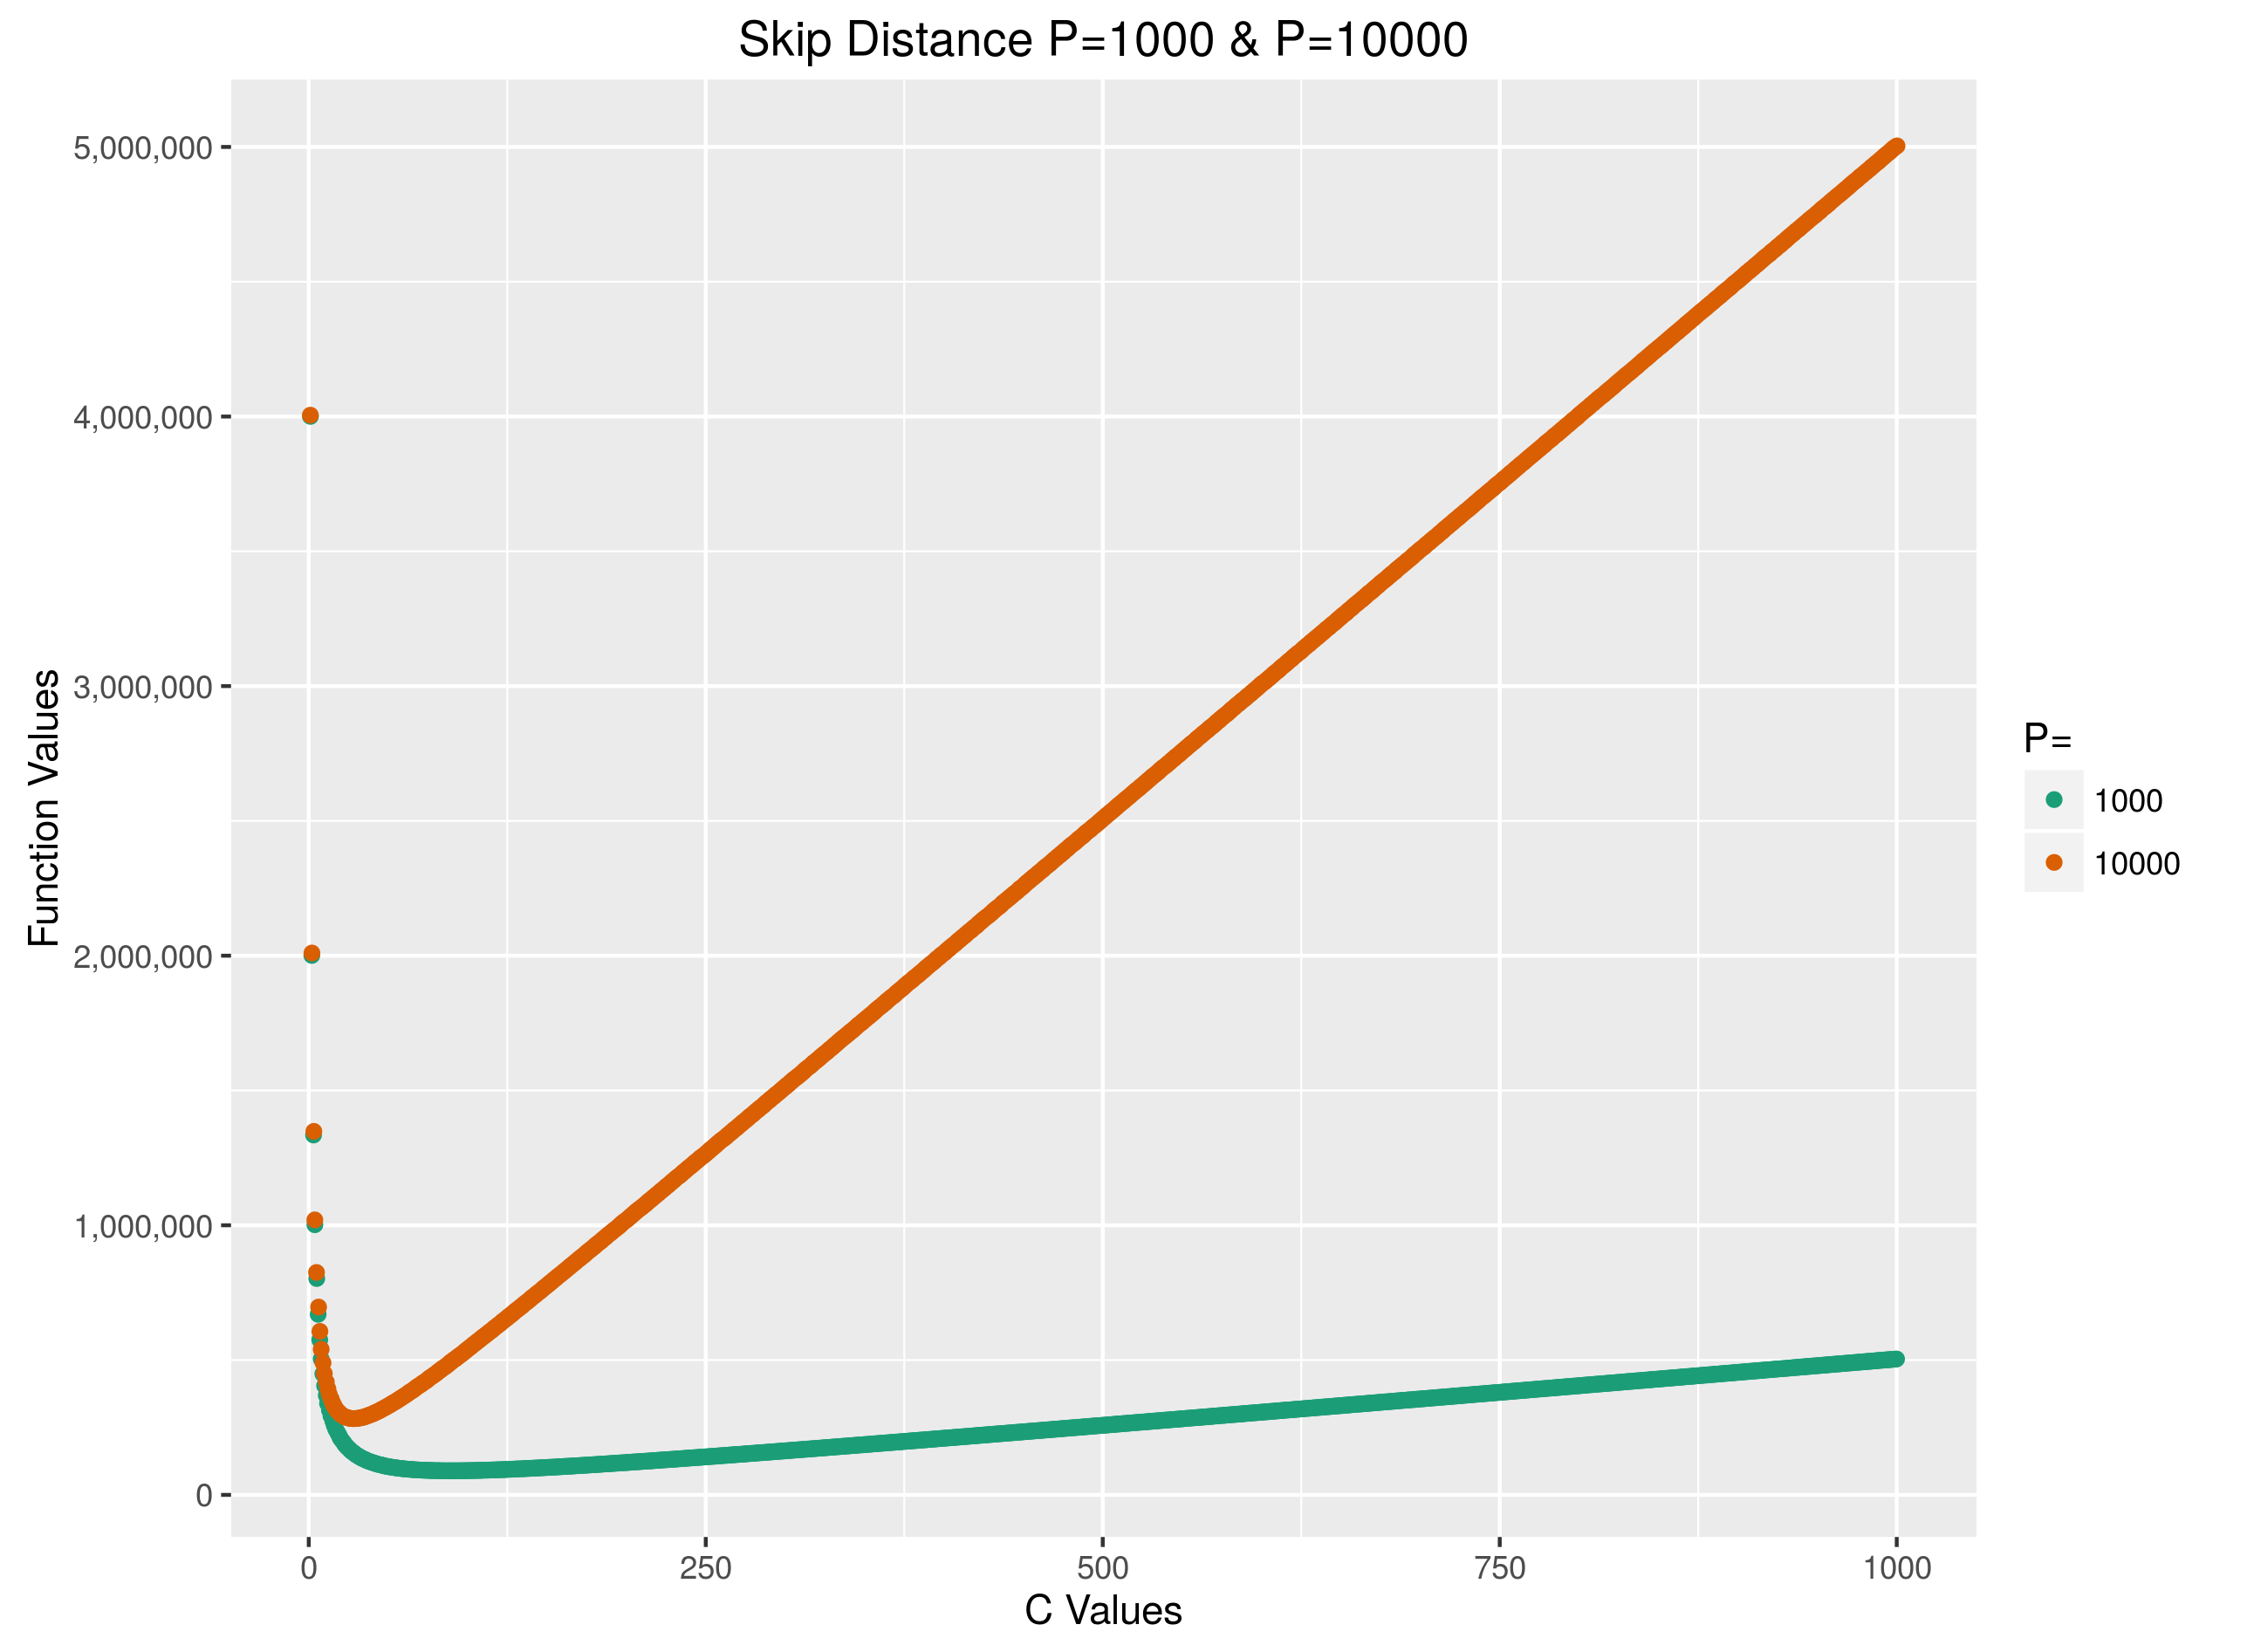
\includegraphics[width=\columnwidth]{code/skipDistanceBoth.png}
\caption{Skip Distance Optimal C Both P Plot}
\label{fig:skbp}
\end{figure}
\begin{figure}[h]
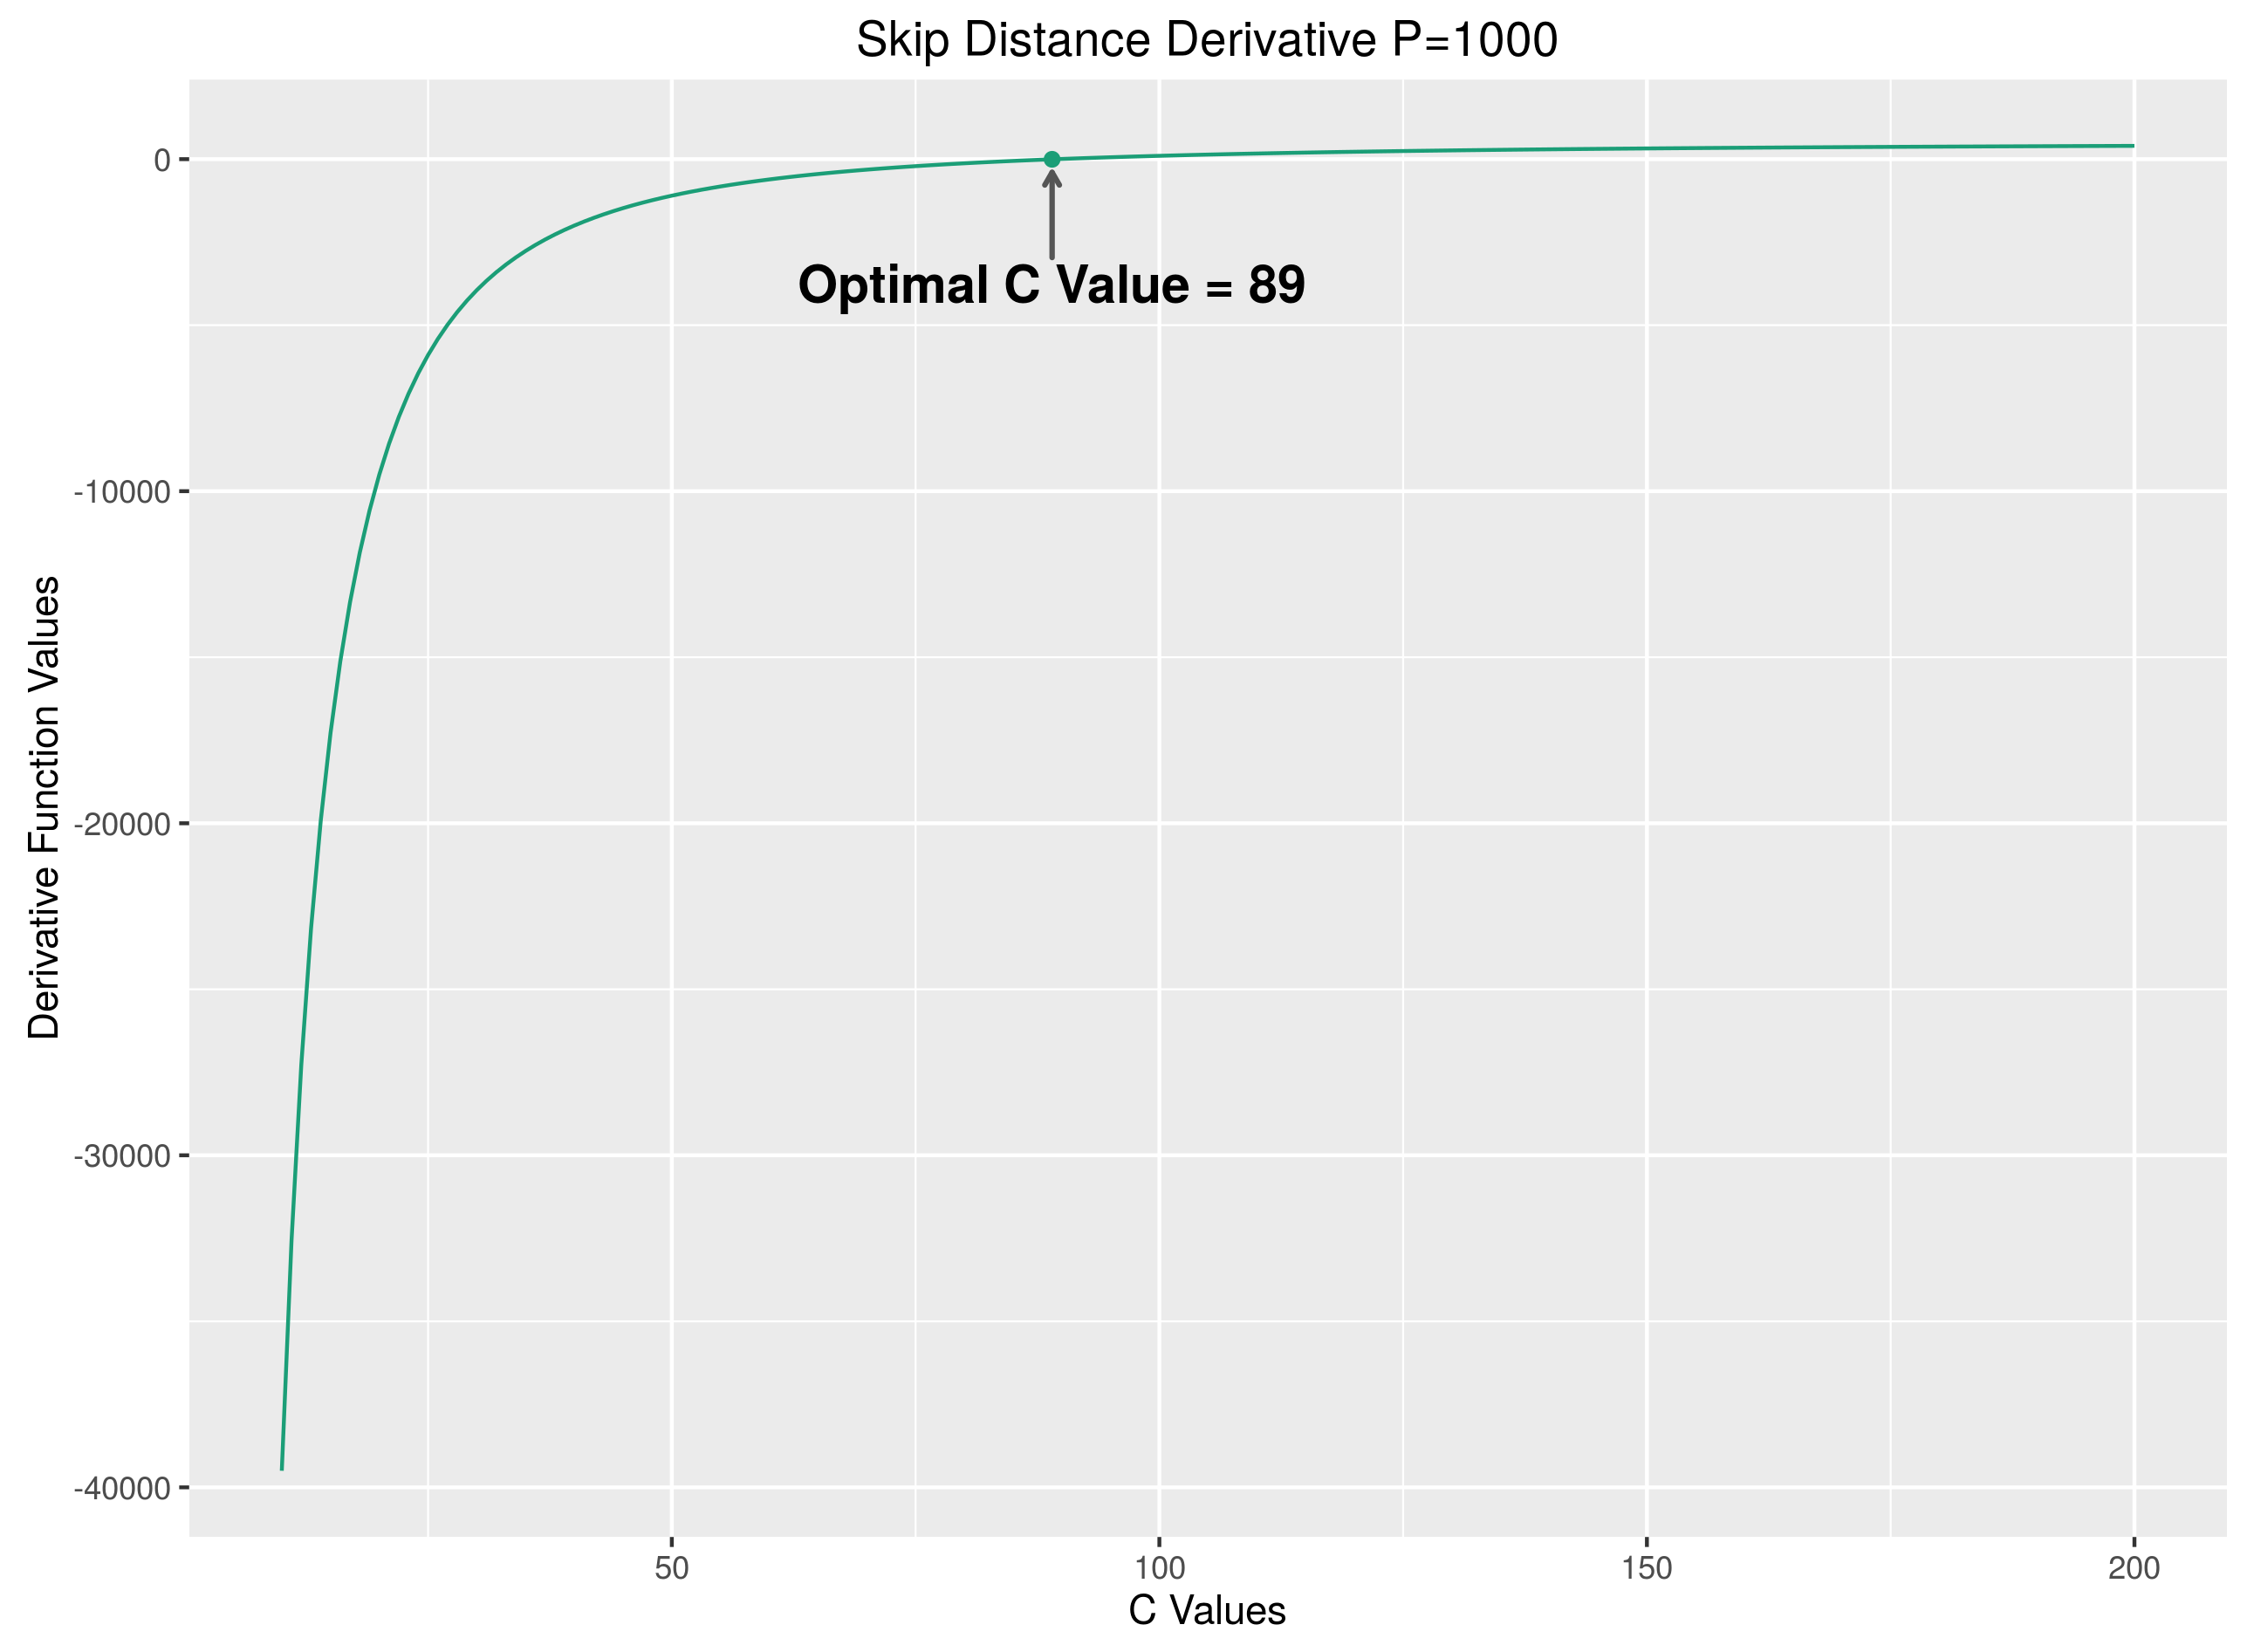
\includegraphics[width=\columnwidth]{code/skipDistanceD.png}
\caption{Skip Distance Derivative P=1000 Plot}
\label{fig:skdp}
\end{figure}
\begin{figure}[h]
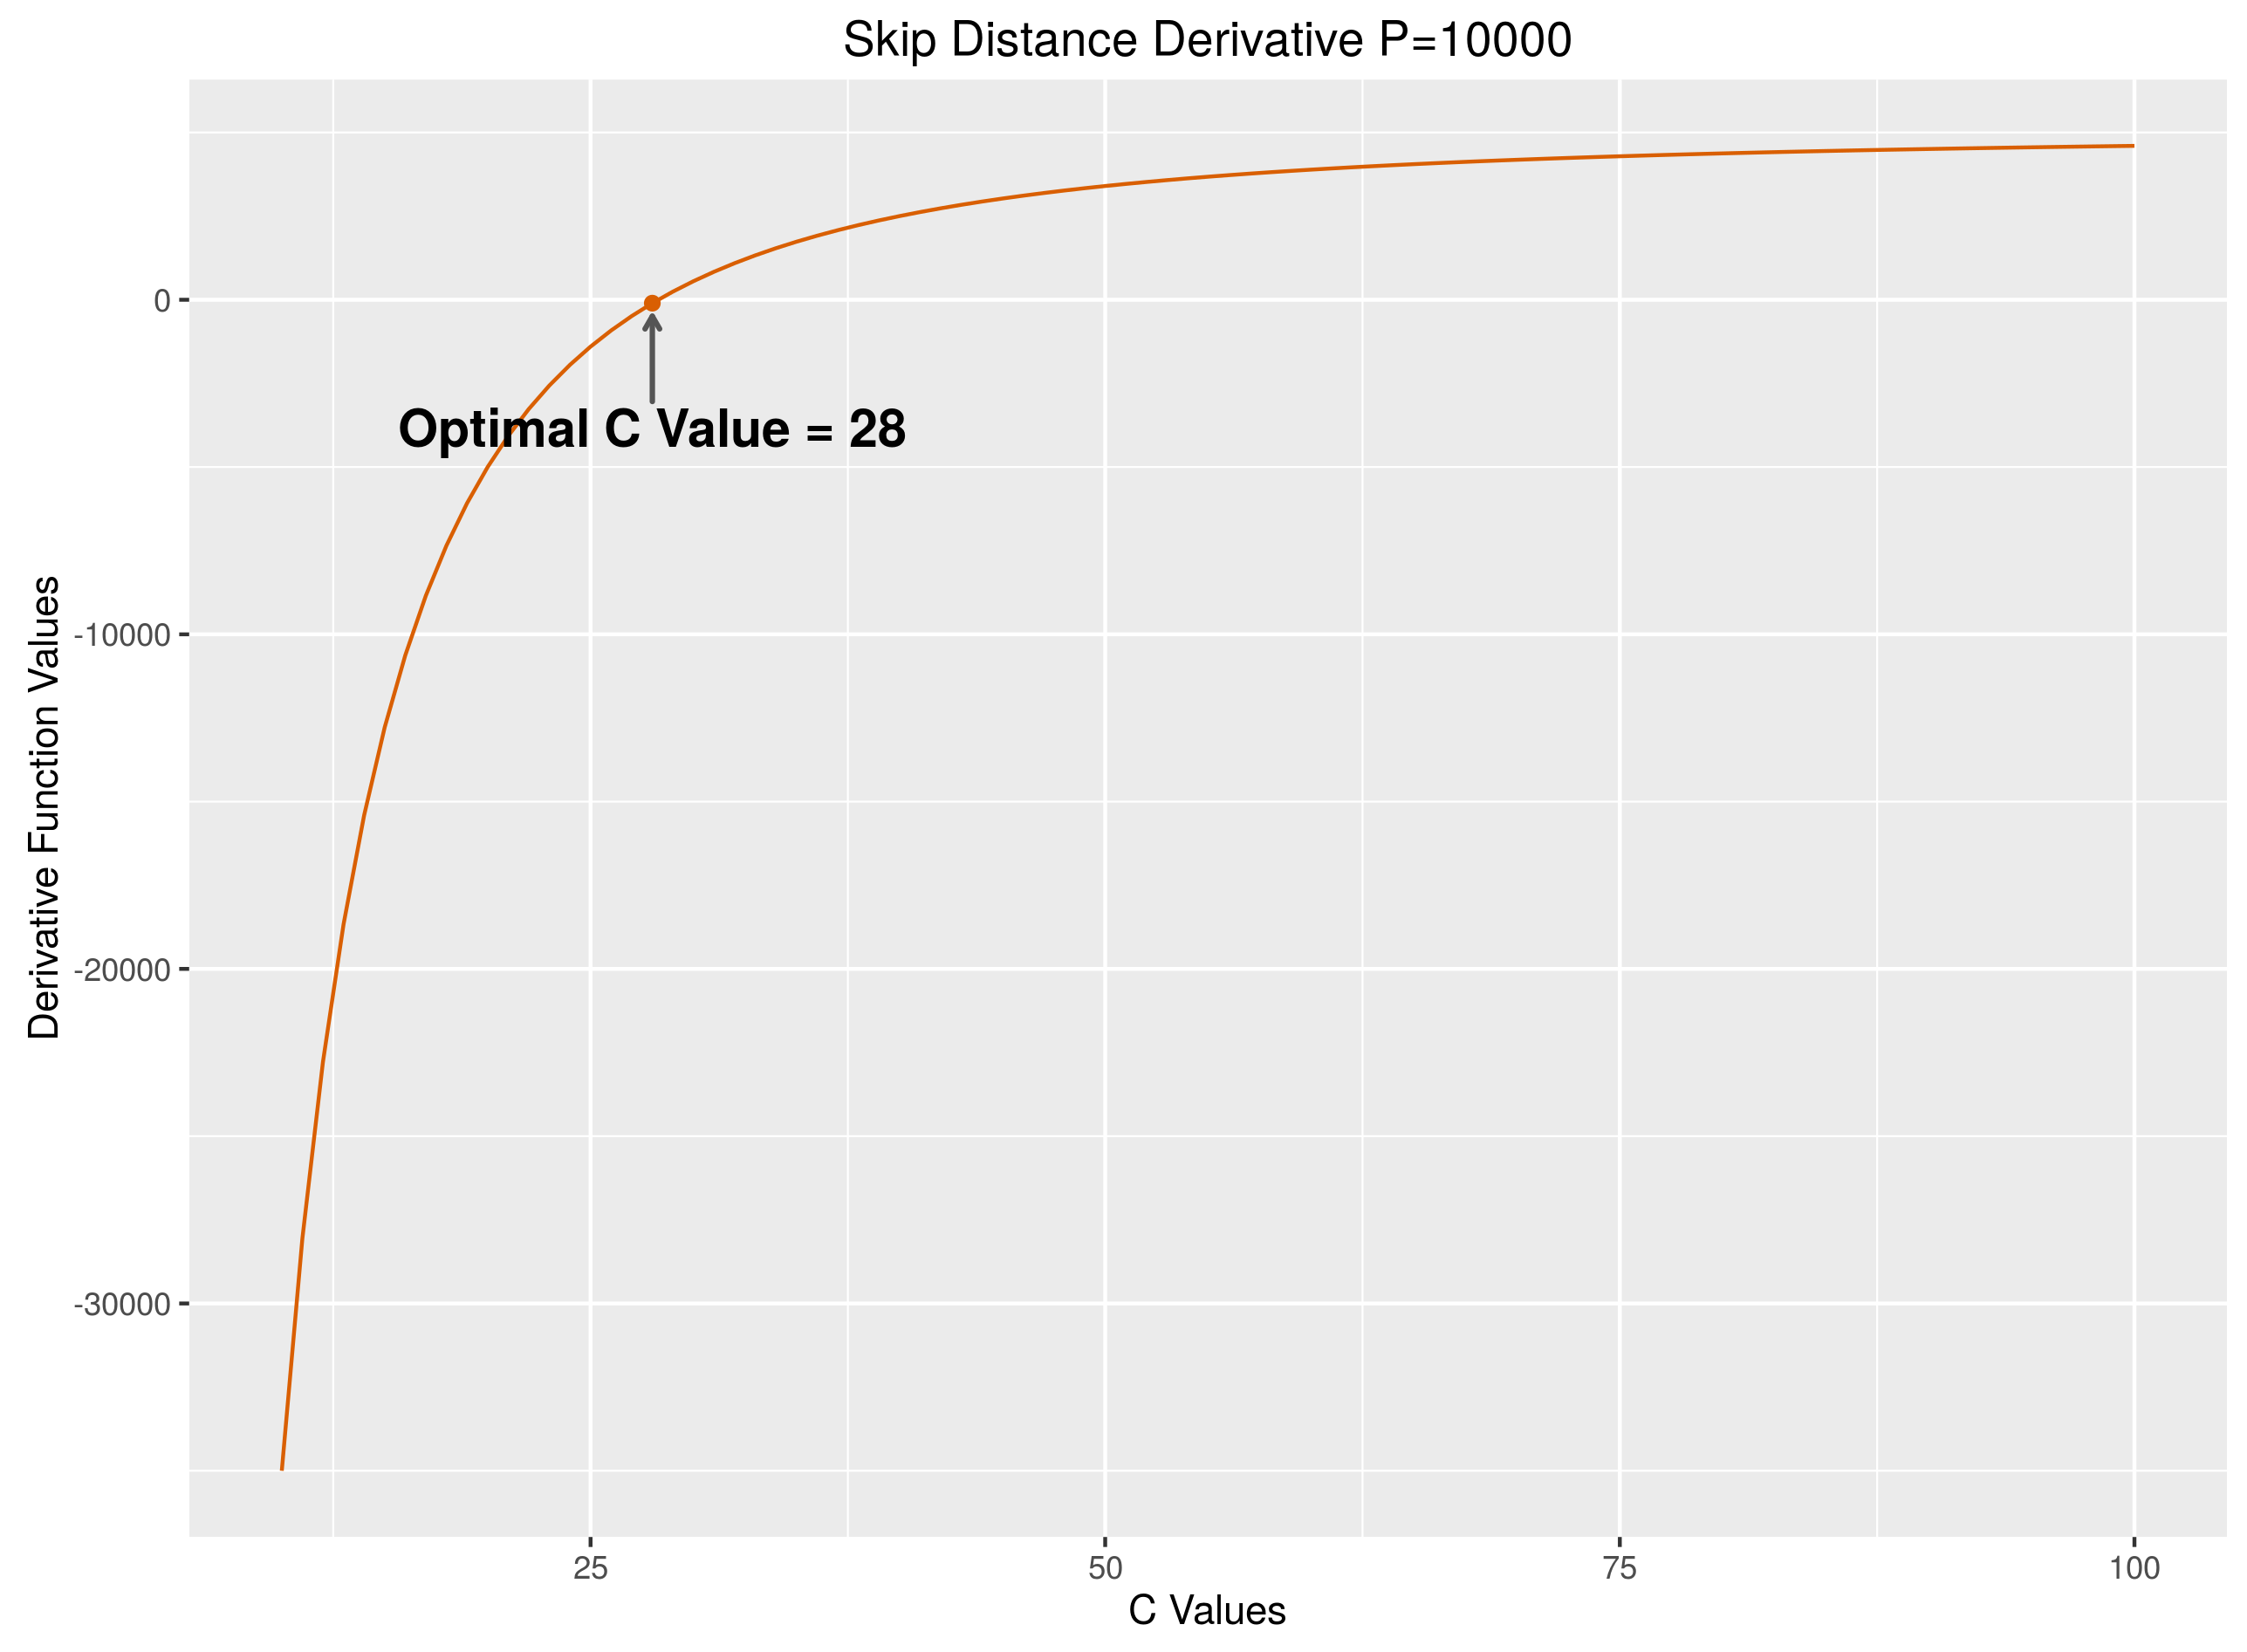
\includegraphics[width=\columnwidth]{code/skipDistanceD2.png}
\caption{Skip Distance Derivative P=10000 Plot}
\label{fig:skdp2}
\end{figure}
\newpage
\clearpage
\begin{code}
	\rcode{code/derivative.R}
	\captionof{listing}{First Derivative Of Skip Distance} \label{code:dsd}
\end{code}
\begin{code}
	\rcode{code/skip_distance.R}
	\captionof{listing}{Skip Distance Plots} \label{code:skip}
\end{code}
\newpage
\begin{code}
	\pycode{code/util.py}
	\captionof{listing}{Util File} \label{code:util}
\end{code}
\end{document}
